\documentclass[10pt,aspectratio=43]{beamer}

\usepackage{tikz}
\usepackage{xcolor}
\usepackage{caption}
\usepackage{subcaption}
\usepackage{bm}
\usetikzlibrary{calc} 
\usepackage{hyperref}
\hypersetup{
    colorlinks=true,
    linkcolor=blue,
    urlcolor=red
}
\usepackage{fontawesome5}

\usetheme{MyStyle}   % loads beamerthemeMyStyle.sty
\setlength{\columnsep}{0pt}

%%%%%%%%%%%%%%%%%%%%%%%%%%%%%%%%%%%%%%%%%%
%%%%%%%%%%%%%%%%%%%%%%%%%%%%%%%%%%%%%%%%%%
%%%%%%%%%%%%%%%%%%%%%%%%%%%%%%%%%%%%%%%%%%

\title{ALERT Track reconstruction \\progress report}
%\title{My Presentation Title}
\author{Felix Touchte Codjo}
\institute{IJCLab}
\date{\today}

\begin{document}

\begin{frame}[plain] % remove header, footer, barre de navigation
\titlepage
\end{frame}

\begin{frame}{Outline}
\tableofcontents
\end{frame}

\section{Kalman Filter Propagator}
\begin{frame}{Kalman Filter Propagator}
    \begin{itemize}
        \item We noticed that the Kalman Filter needed a lot of iterations in order to converge
        \item That increased the computation time
        \item We improved the Propagator algorithm
            \begin{itemize}
                \item cleaning, object merging
                \item better management of the step size of the RK4
            \end{itemize}
        \item We reduced the initial computing time by a factor 8
    \end{itemize}

    \vspace{0.2cm}

    \centering
    \begin{tikzpicture}
            \node[anchor=south west, inner sep=0] (image) at (0,0) {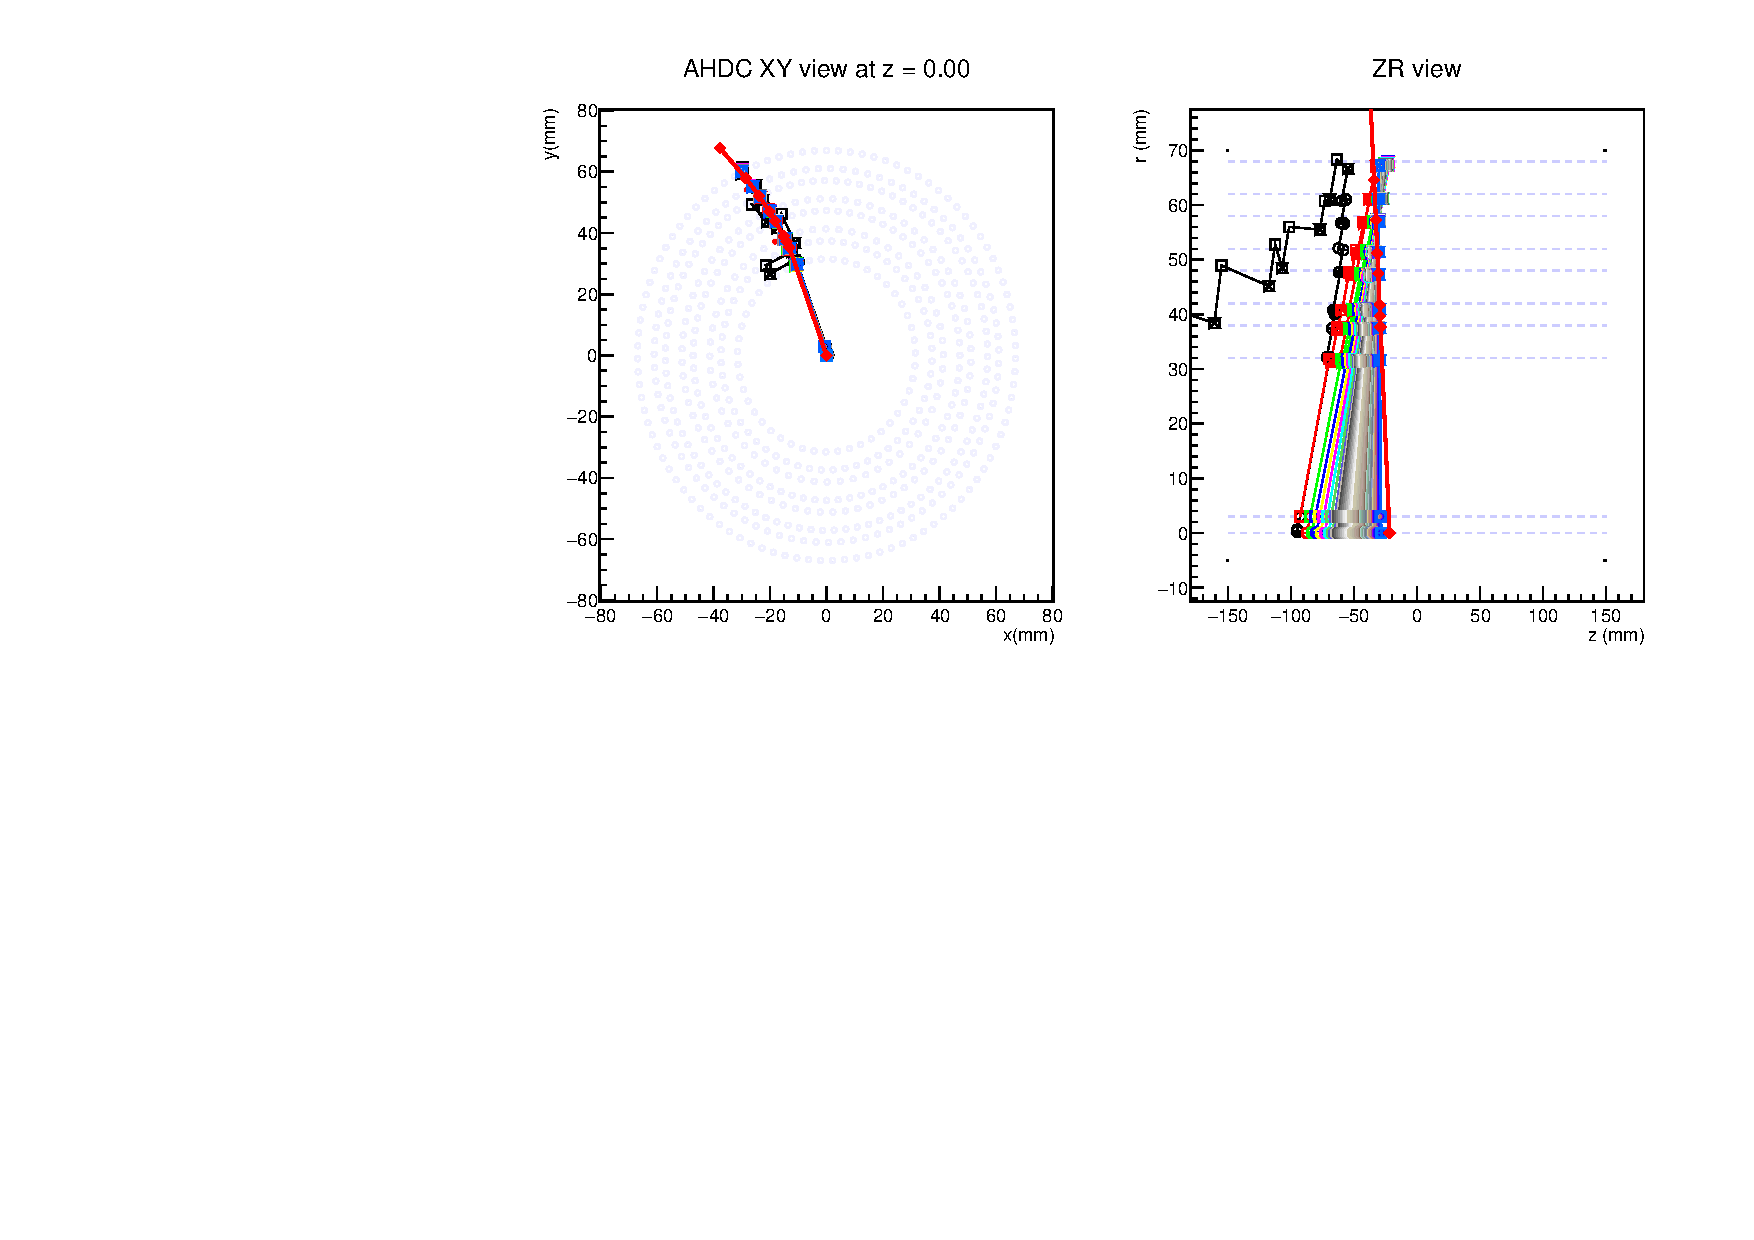
\includegraphics[width=0.8\textwidth]{figures/kalman-filter-monitoring-simu.pdf}};
            % Option : système de coordonnées relatif (0 à 1)
            \begin{scope}[x={(image.south east)}, y={(image.north west)}]
                %\node [red] at (0.7,0.6) {\tiny after};
                \draw [<-, red] (0.73,0.4) -- (0.8,0.45) node [right] {\tiny mc trajectory};
                \draw [->, blue] (0.63,0.17) -- node [below, midway] {\tiny Niter} (0.74,0.17);
            \end{scope}
        \end{tikzpicture}
    

\end{frame}

\section{Use more than 2 hits per layer}
\begin{frame}{Use more than 2 hits per layer}
    \begin{itemize}
        \item Before, the Kalman Filter only managed one hit per layer
        \item Having two hits on the layer is extra information (see 1-hit only track versus 2-hit correction track; residual before and after for simulation)
        \item However, now that we can have more than 2 hits per layer, we have to take into the deposited energy of the hits to balance their effect
        
    \end{itemize}
    \vspace{0.2cm}

    %Managing more than two hits on the same layer gives extra information. In this example, the low deposited energy (blue filled circle) on the 2-hit cluster of the layer 3 (numerotation going for the inner layer to the outer layer) indicates an important shift of the trajectory towards the left direction. This is confirmed as in the upper layers the deposited energy of the left hit of the 2-hit cluster become bigger. The dashed black arrow is the trajectory with one hit only, while the the blue arrow is the trajectory with two hits. The points have been fitted with a circle. We can see that the 2 hit correction has a more consistent projection at the center of the detector. 

    %The hits are given to the Kalman in the following order: from inner layer to outer layer and from right to left (see figure).
    % We take into account the deposited energy in the distance resolution

    \centering
    \begin{minipage}{0.45\textwidth}
        %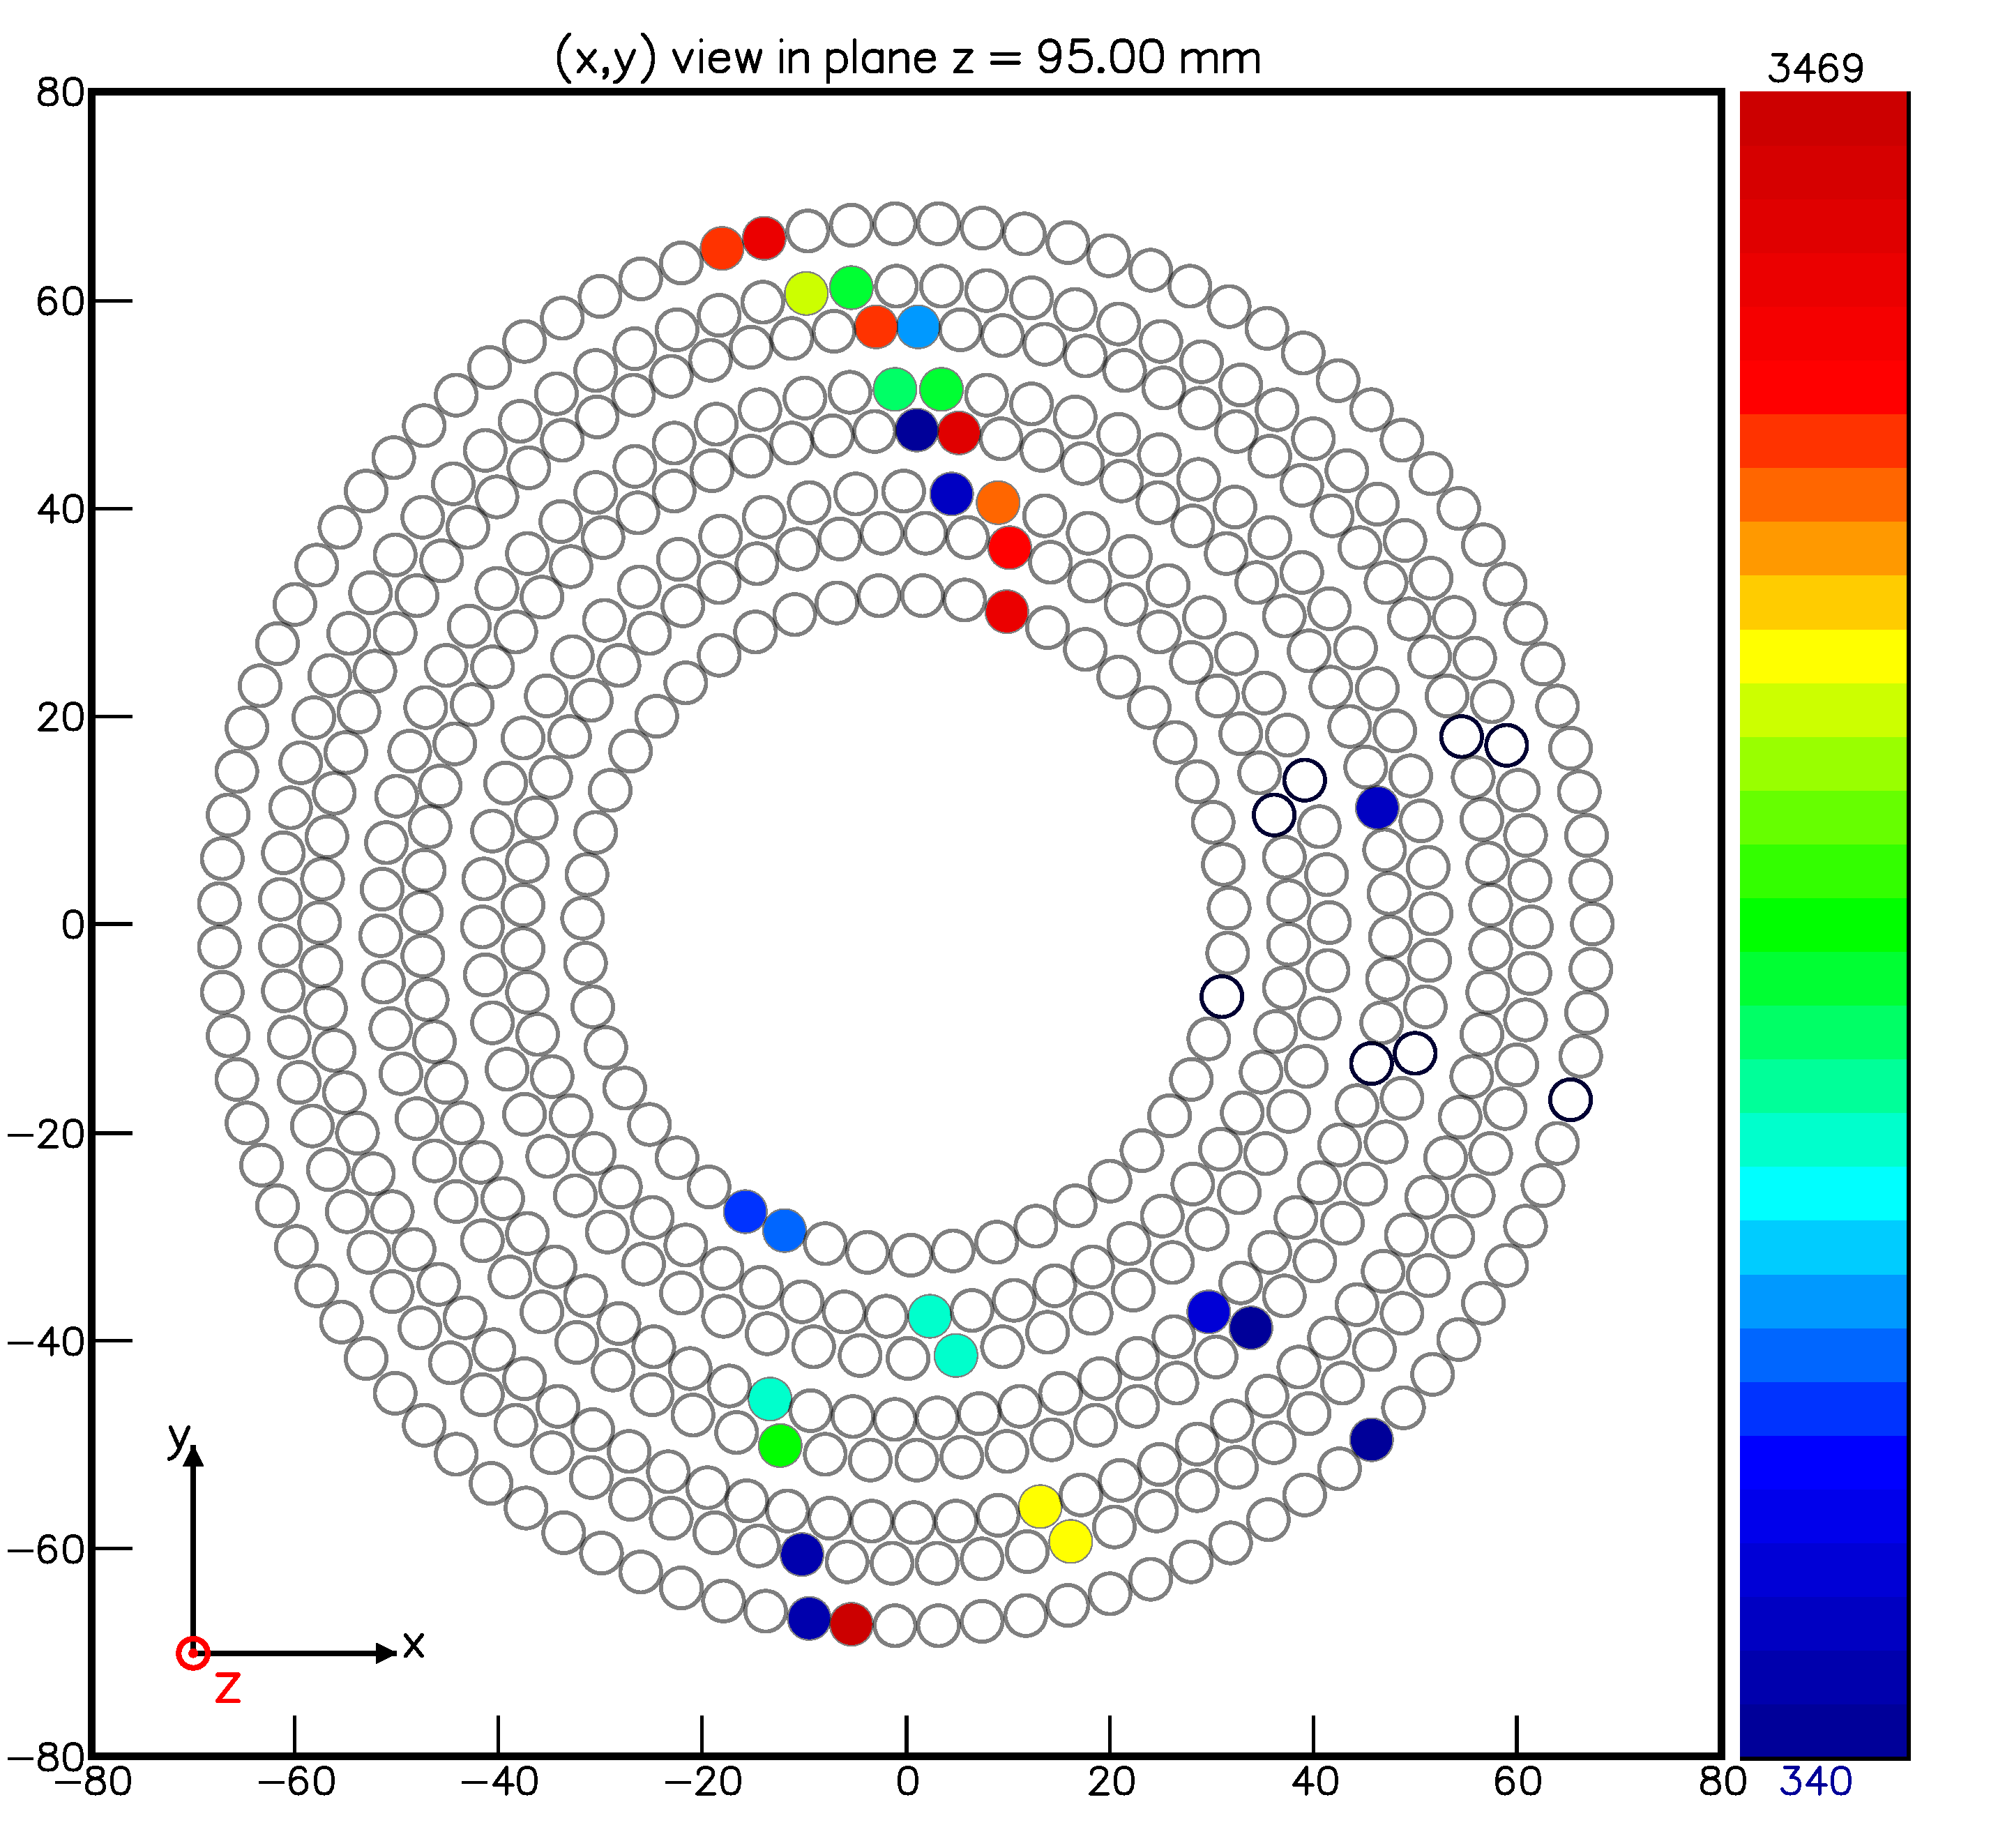
\includegraphics[width=\linewidth]{figures/event_display_use_all_hits_in_kf.pdf}
        \begin{tikzpicture}
            \node[anchor=south west, inner sep=0] (image) at (0,0) {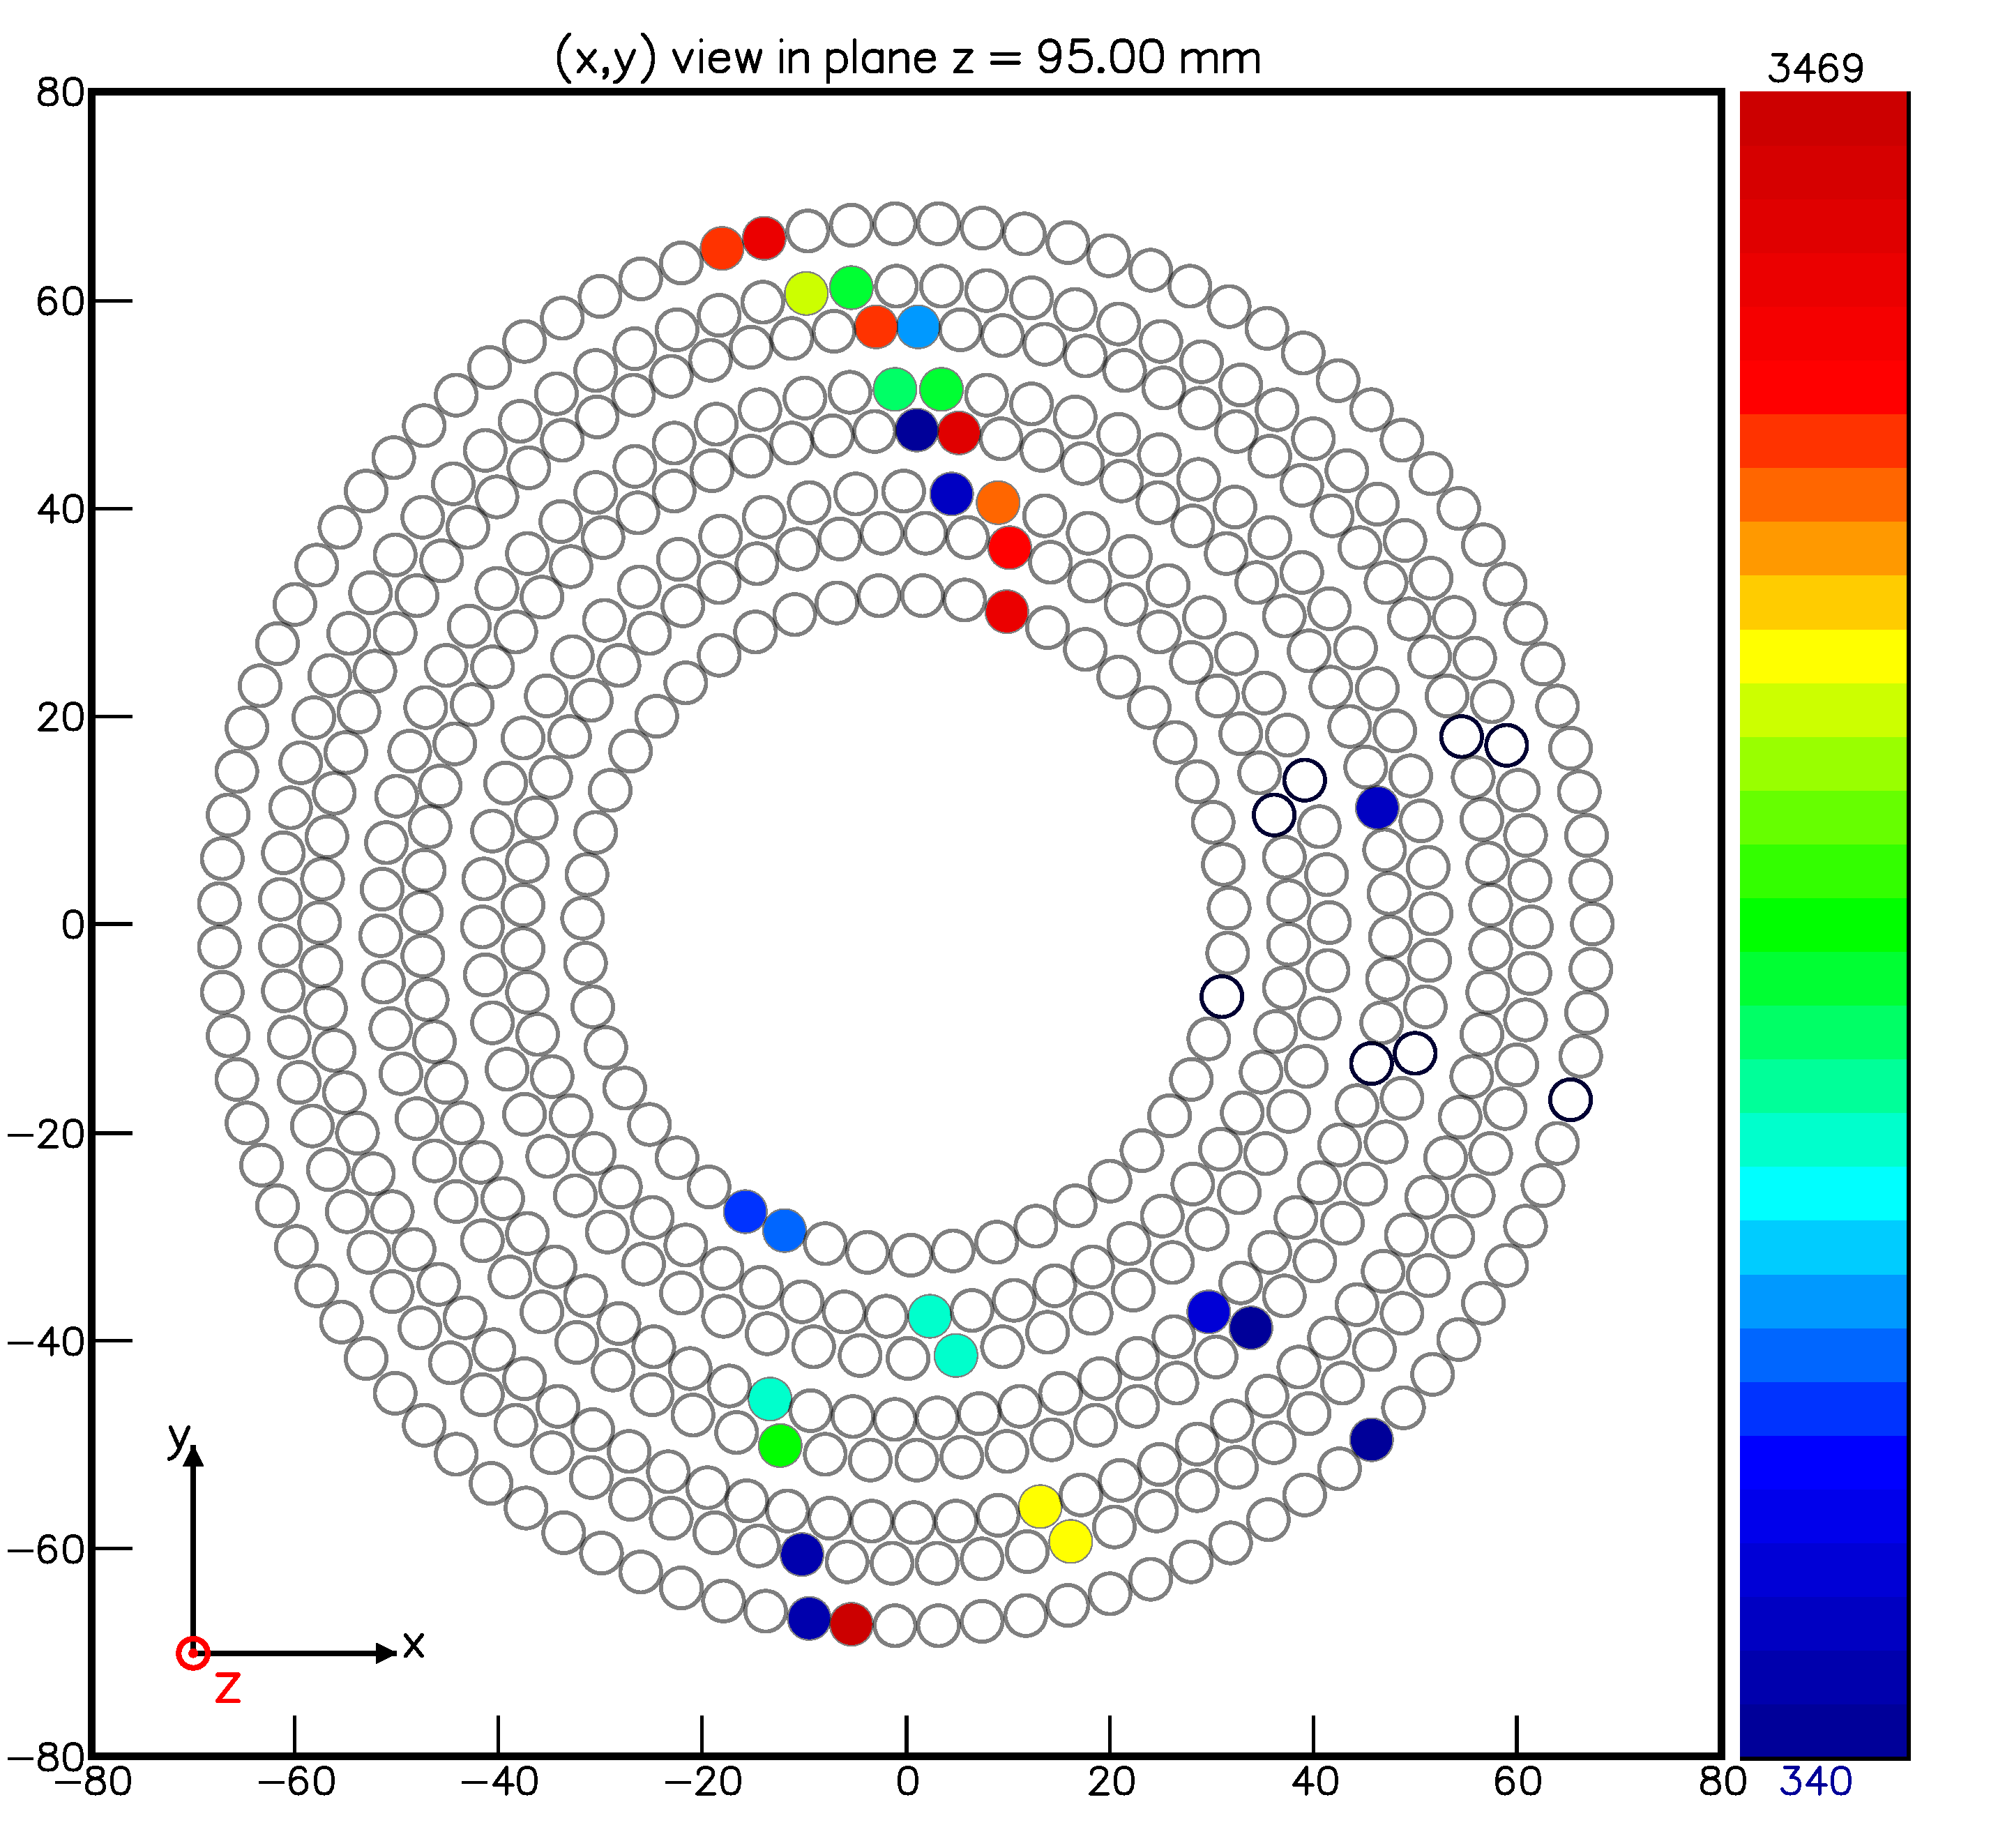
\includegraphics[width=\linewidth]{figures/event_display_use_all_hits_in_kf.pdf}};
            % Option : système de coordonnées relatif (0 à 1)
            \begin{scope}[x={(image.south east)}, y={(image.north west)}]
                % --- points A, B, C
                \def\xA{0.50}
                \def\yA{0.66}
                \def\xB{0.48}
                \def\yB{0.76}
                \def\xC{0.38}
                \def\yC{0.87}
                % --- Calcul du déterminant ---
                \pgfmathsetmacro{\D}{2*(\xA*(\yB-\yC) + \xB*(\yC-\yA) + \xC*(\yA-\yB))}
                % --- Centre du cercle ---
                \pgfmathsetmacro{\xc}{
                ((\xA*\xA+\yA*\yA)*(\yB-\yC) +
                (\xB*\xB+\yB*\yB)*(\yC-\yA) +
                (\xC*\xC+\yC*\yC)*(\yA-\yB))/\D
                }
                \pgfmathsetmacro{\yc}{
                ((\xA*\xA+\yA*\yA)*(\xC-\xB) +
                (\xB*\xB+\yB*\yB)*(\xA-\xC) +
                (\xC*\xC+\yC*\yC)*(\xB-\xA))/\D
                }
                % --- Rayon ---
                \pgfmathsetmacro{\r}{sqrt((\xA-\xc)^2 + (\yA-\yc)^2)}
                % --- Angles pour l'arc ---
                \pgfmathsetmacro{\angleA}{atan2(\yA-\yc,\xA-\xc)-44}
                \pgfmathsetmacro{\angleC}{atan2(\yC-\yc,\xC-\xc)+15}
                % arc entre A et C
                \draw[line width=0.5pt,black,dashed,->] (\xc,\yc) ++(\angleA:\r) arc (\angleA:\angleC:\r) node [right, xshift=4, yshift=3]{\tiny 1-hit only};
            \end{scope}
            \begin{scope}[x={(image.south east)}, y={(image.north west)}]
                % --- points A, B, C
                \def\xA{0.50}
                \def\yA{0.66}
                \def\xB{0.47}
                \def\yB{0.77}
                \def\xC{0.37}
                \def\yC{0.87}
                % --- Calcul du déterminant ---
                \pgfmathsetmacro{\D}{2*(\xA*(\yB-\yC) + \xB*(\yC-\yA) + \xC*(\yA-\yB))}
                % --- Centre du cercle ---
                \pgfmathsetmacro{\xc}{
                ((\xA*\xA+\yA*\yA)*(\yB-\yC) +
                (\xB*\xB+\yB*\yB)*(\yC-\yA) +
                (\xC*\xC+\yC*\yC)*(\yA-\yB))/\D
                }
                \pgfmathsetmacro{\yc}{
                ((\xA*\xA+\yA*\yA)*(\xC-\xB) +
                (\xB*\xB+\yB*\yB)*(\xA-\xC) +
                (\xC*\xC+\yC*\yC)*(\xB-\xA))/\D
                }
                % --- Rayon ---
                \pgfmathsetmacro{\r}{sqrt((\xA-\xc)^2 + (\yA-\yc)^2)}
                % --- Angles pour l'arc ---
                \pgfmathsetmacro{\angleA}{atan2(\yA-\yc,\xA-\xc)-40}
                \pgfmathsetmacro{\angleC}{atan2(\yC-\yc,\xC-\xc)+25}
                % arc entre A et C
                \draw[line width=0.5pt,blue,->] (\xc,\yc) ++(\angleA:\r) arc (\angleA:\angleC:\r) node [left]{\tiny 2-hit correction};
                \draw [red] (0.45,0.5) circle [radius=1pt] node [right] {\tiny center};
            \end{scope}
        \end{tikzpicture}
    \end{minipage}
    \begin{minipage}{0.39\textwidth}
        %
\includegraphics[width=\linewidth]{figures/residual_before_use_all_hits_residual.pdf}
        %
\includegraphics[width=\linewidth]{figures/residual_after_use_all_hits_residual.pdf}
        \begin{tikzpicture}
            \node[anchor=south west, inner sep=0] (image) at (0,0) {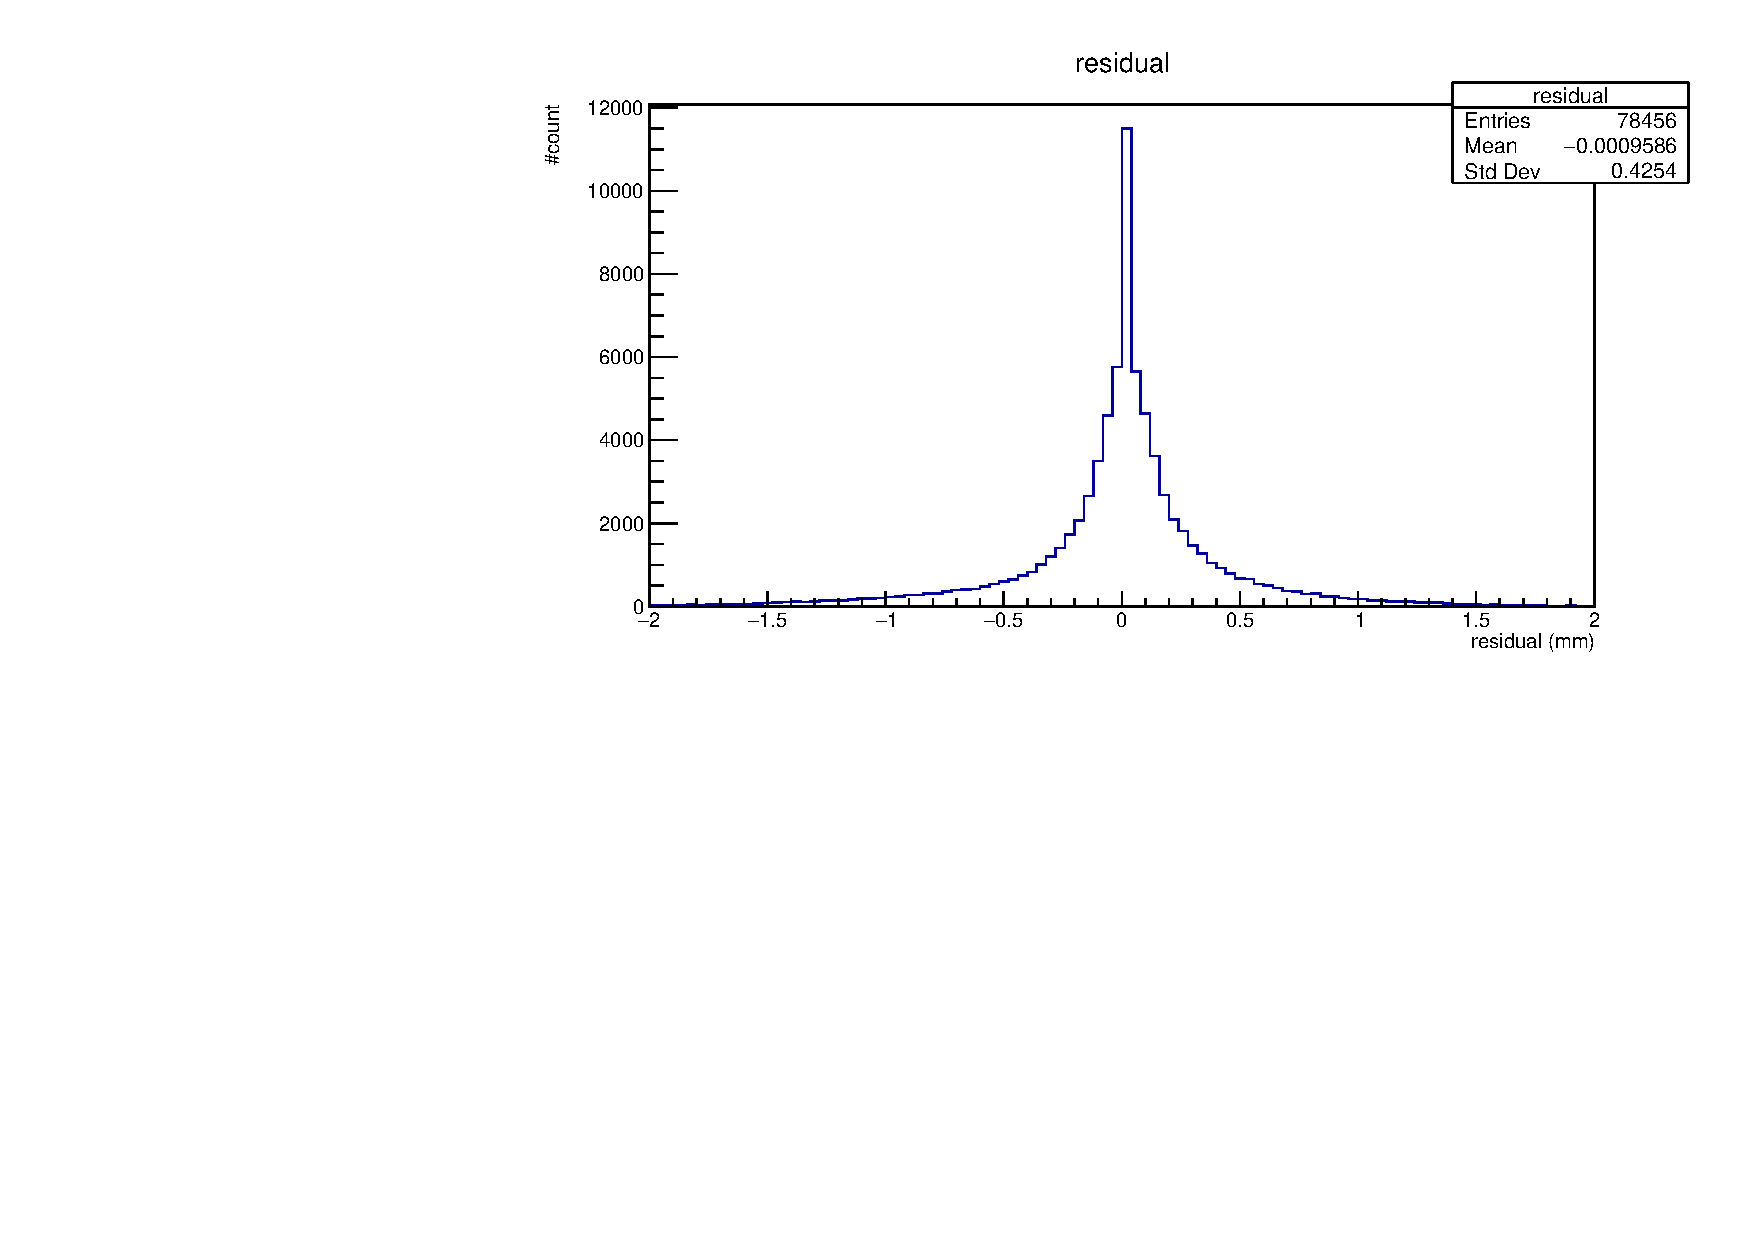
\includegraphics[width=\linewidth]{figures/residual_before_use_all_hits_residual_simu.pdf}};
            % Option : système de coordonnées relatif (0 à 1)
            \begin{scope}[x={(image.south east)}, y={(image.north west)}]
                \node [red] at (0.7,0.6) {\tiny before};
            \end{scope}
        \end{tikzpicture}
        \begin{tikzpicture}
            \node[anchor=south west, inner sep=0] (image) at (0,0) {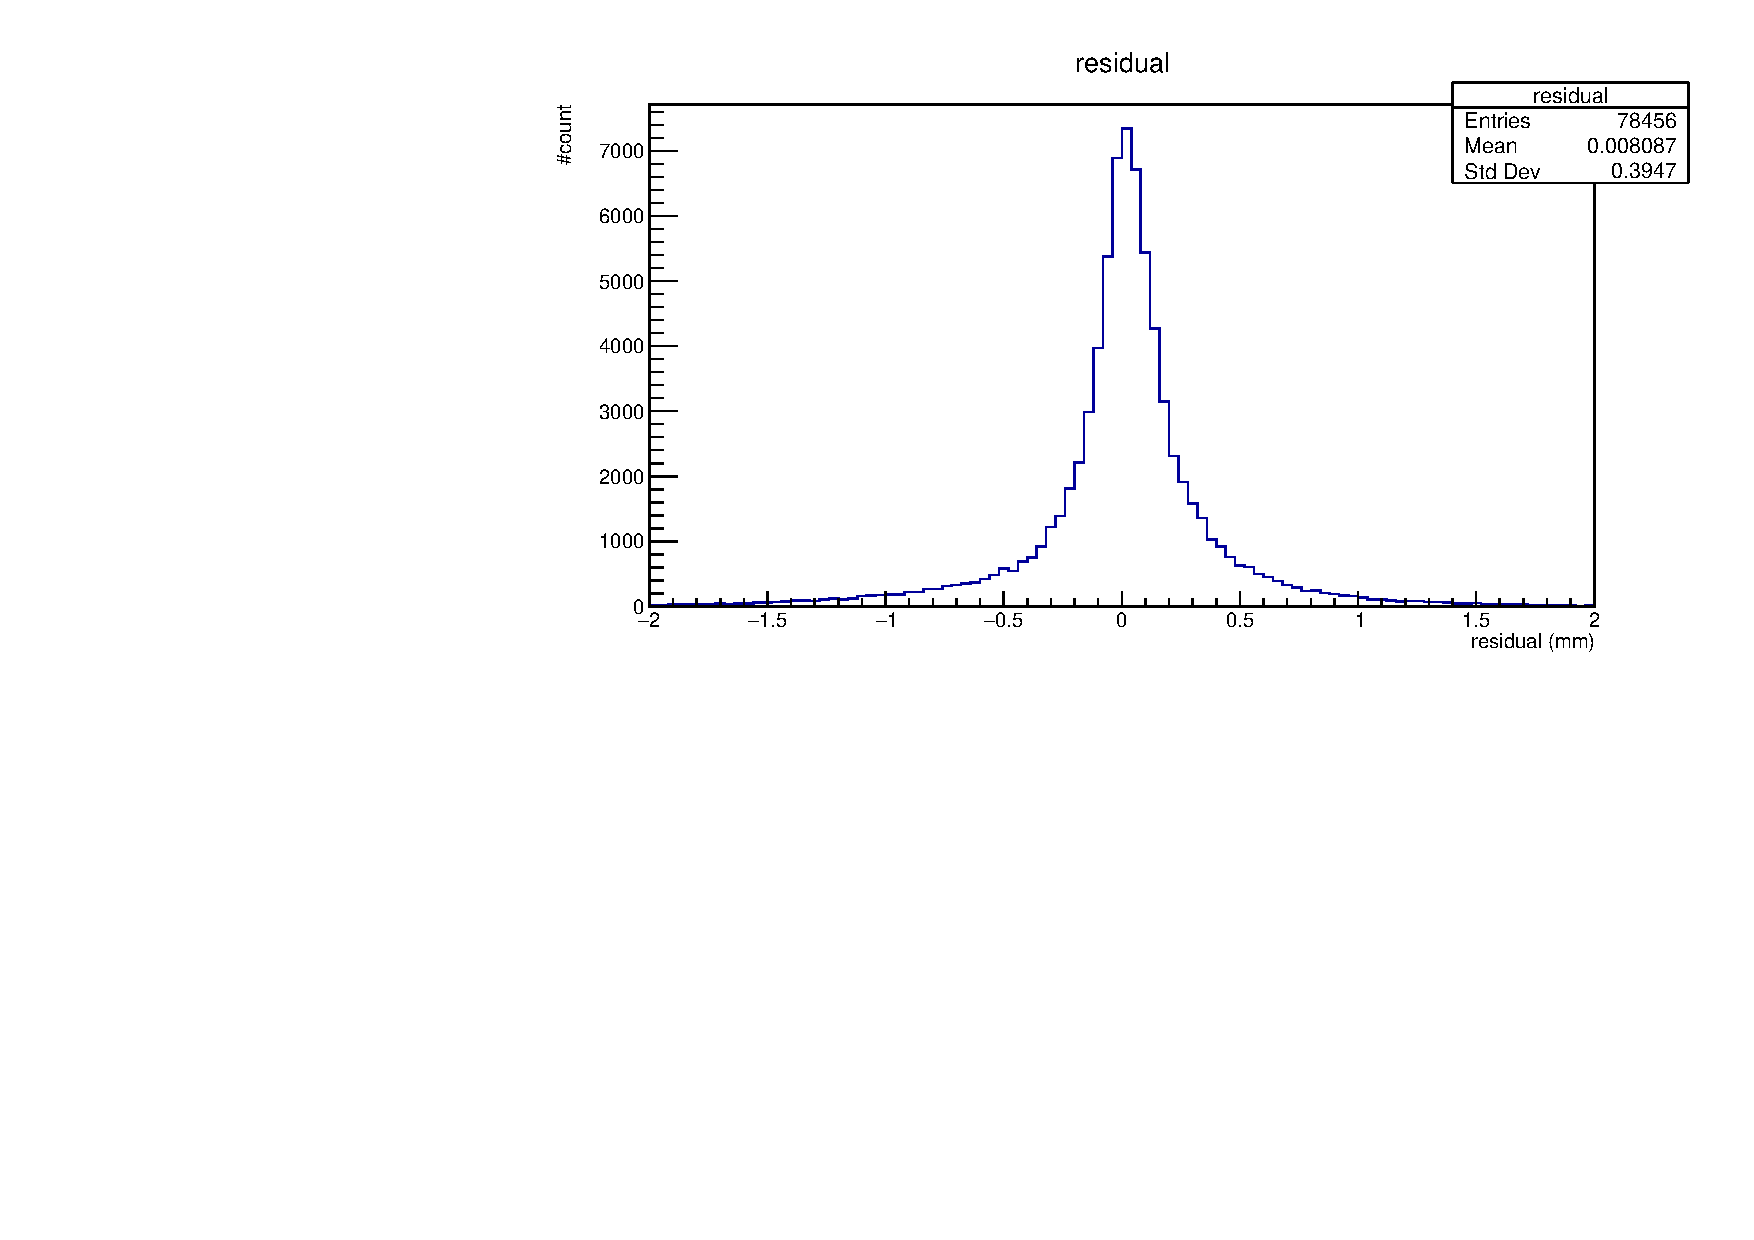
\includegraphics[width=\linewidth]{figures/residual_after_use_all_hits_residual_simu.pdf}};
            % Option : système de coordonnées relatif (0 à 1)
            \begin{scope}[x={(image.south east)}, y={(image.north west)}]
                \node [red] at (0.7,0.6) {\tiny after};
            \end{scope}
        \end{tikzpicture}
        
    \end{minipage}

\end{frame}

\section{Distance resolution with ADC and Time}
\begin{frame}{Distance resolution with ADC and Time}
    \begin{itemize}
        \item The measurements for the AHDC hits in the Kalman Filter are the distances with respect to the wires provided by the timing information of their signals
        \item We make the measurement noise varies with ADC and time (fine-tuning remain to be done). Before it was a constant value.
    \end{itemize}

    % The measurement noise is the measured resoltion of the the tracking. It is given by the width of the residual distribution. Instead of using aa constant value, we make it dependent on ADC and time. Due to low statistics for big ADC and Time, this first implementation performed a fit respectively between 0 and 1000 and 0 and 100.

    \vspace{0.2cm}
    \centering

    \begin{minipage}{0.38\textwidth}
        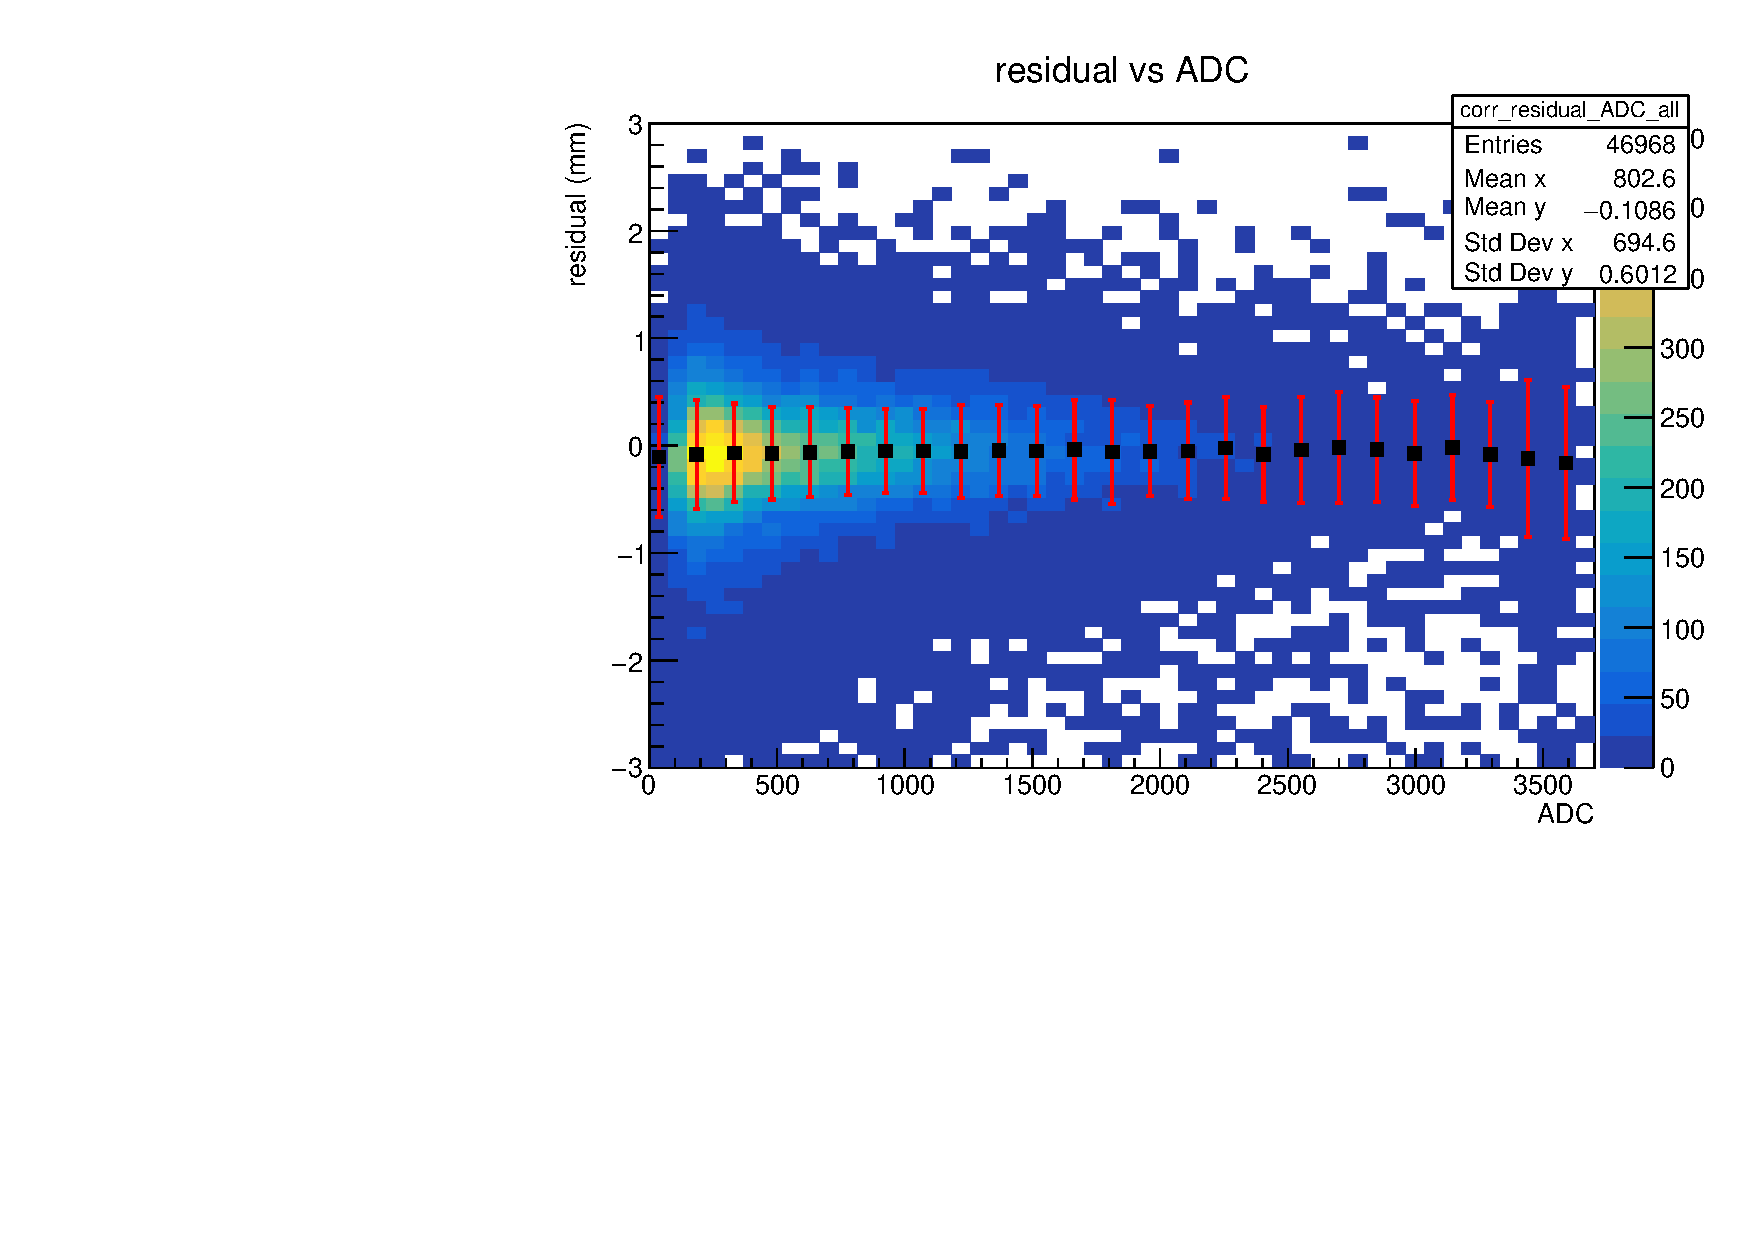
\includegraphics[width=\linewidth]{figures/residual_vs_ADC_2D.pdf}
        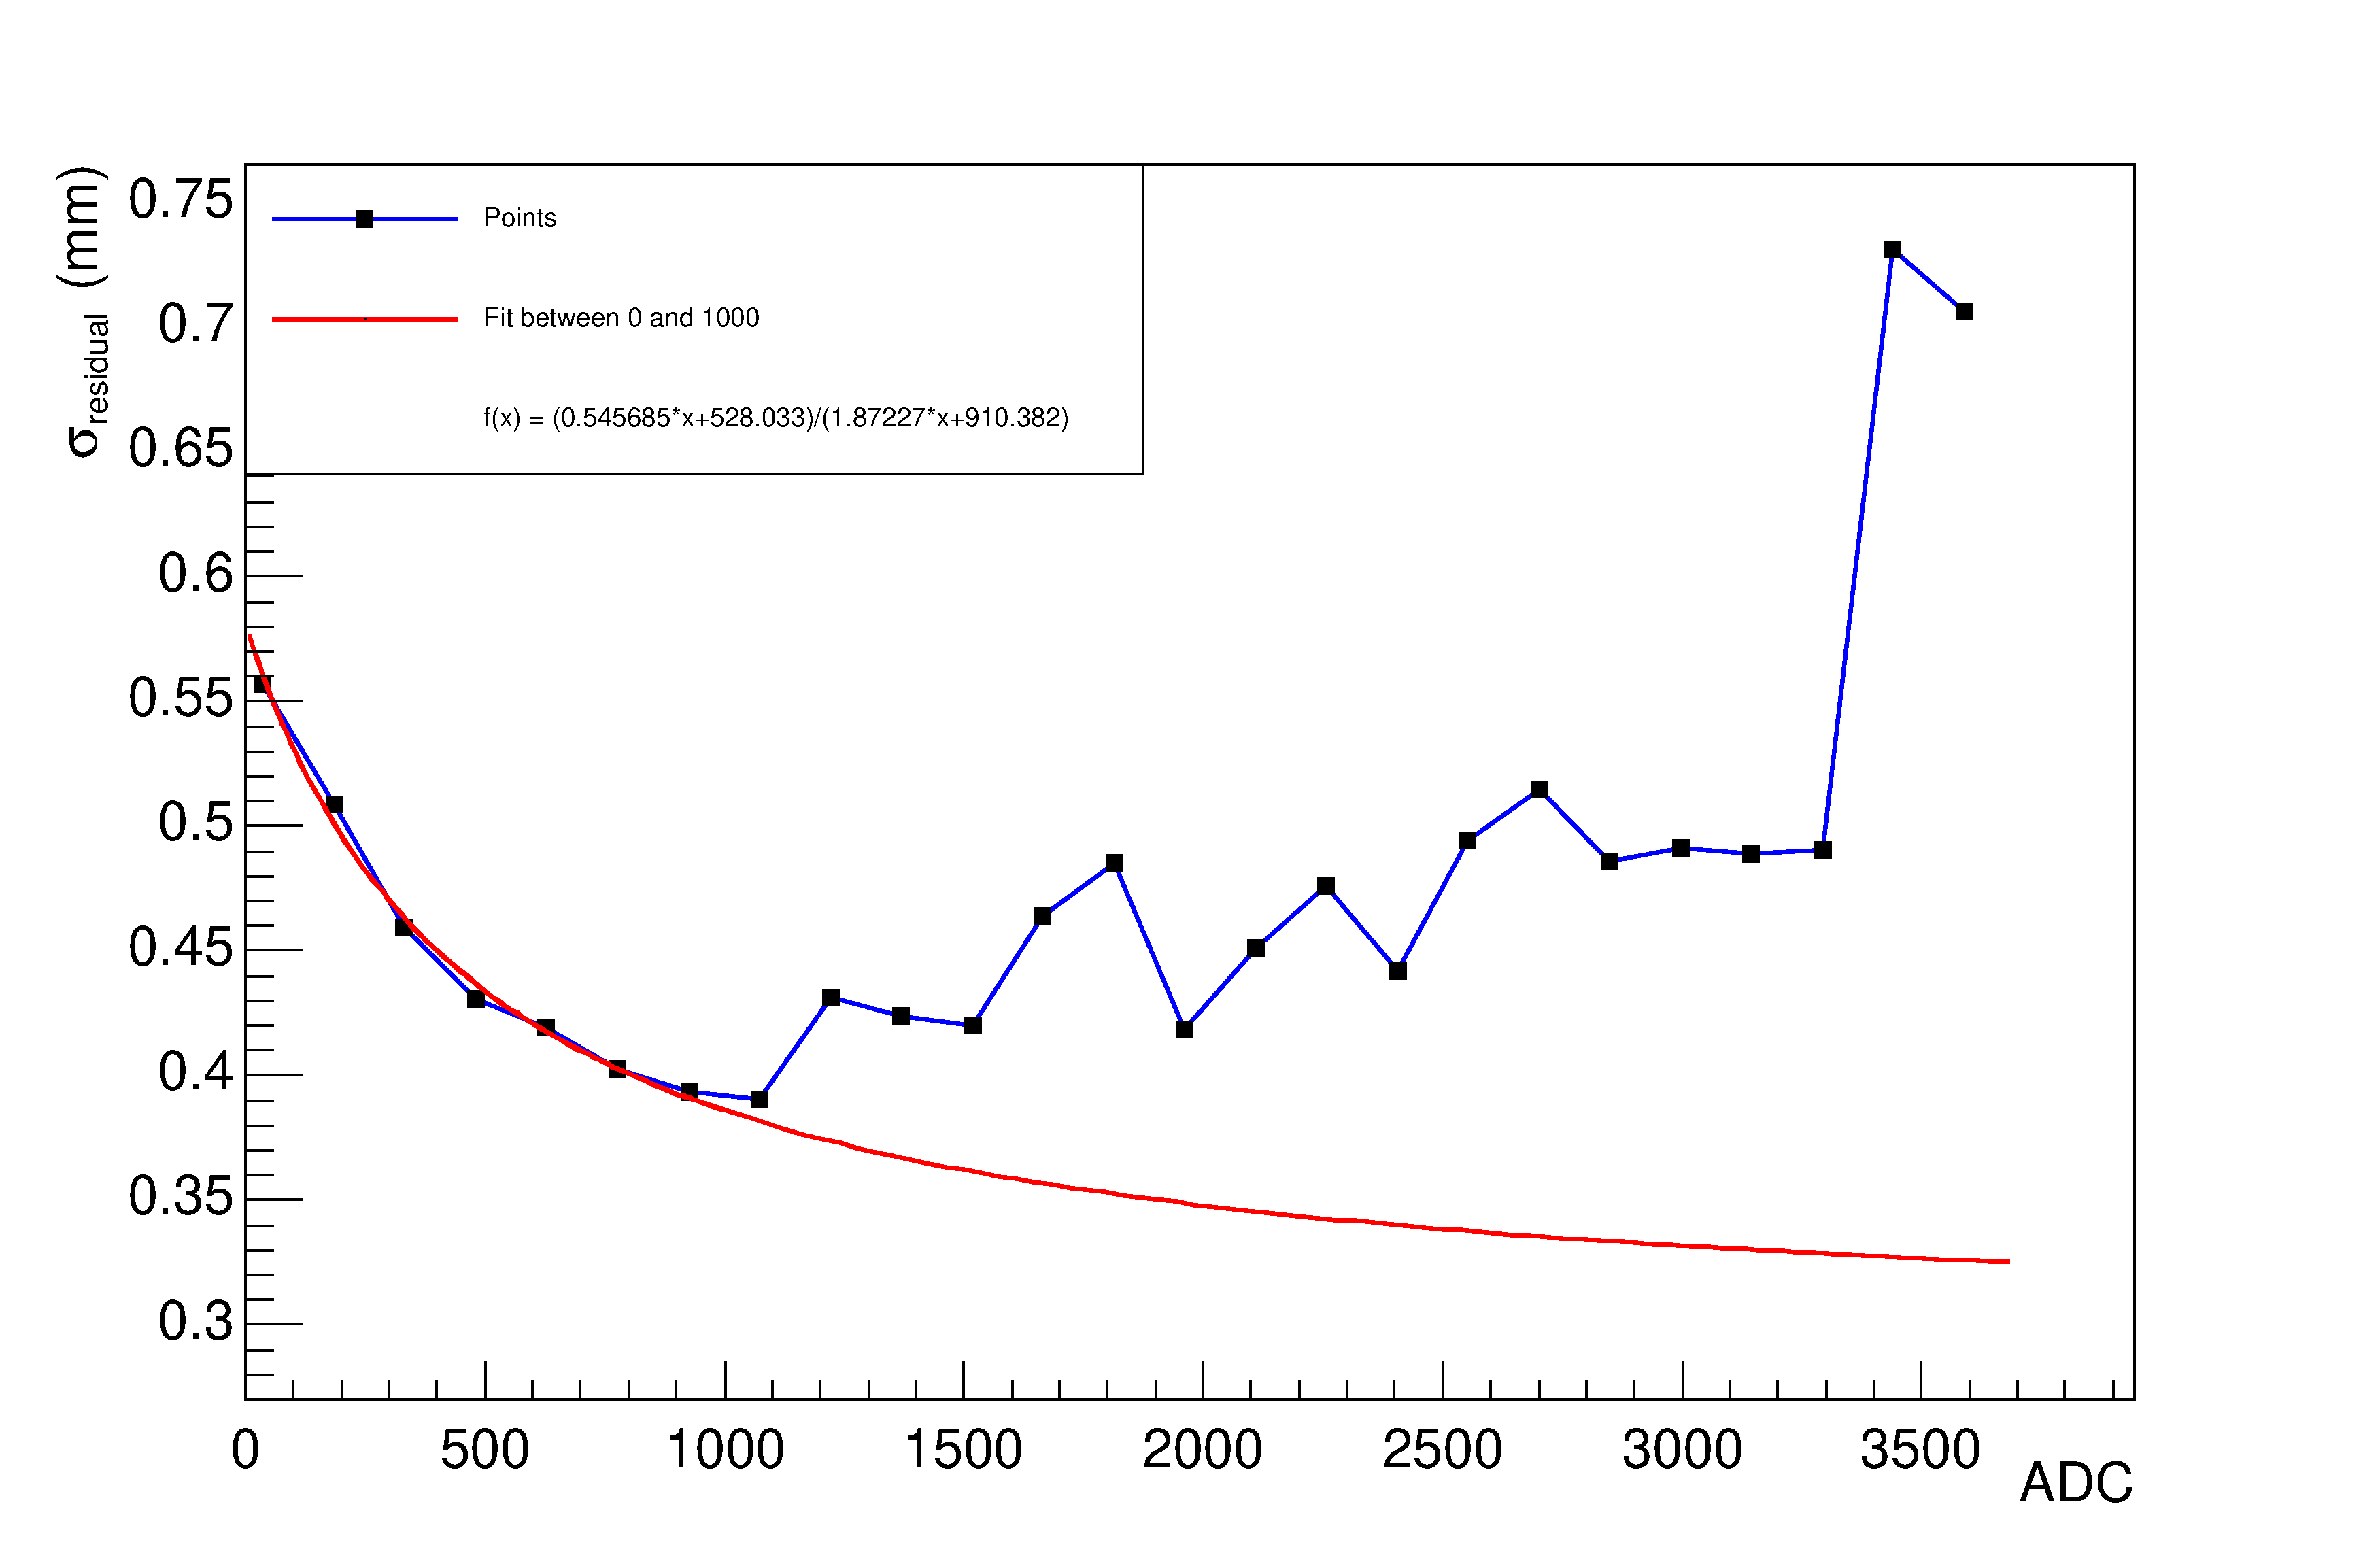
\includegraphics[width=\linewidth]{figures/resolution_residual_on_ADC.pdf}
    \end{minipage}
    \vspace{0.5cm}
    \begin{minipage}{0.38\textwidth}
        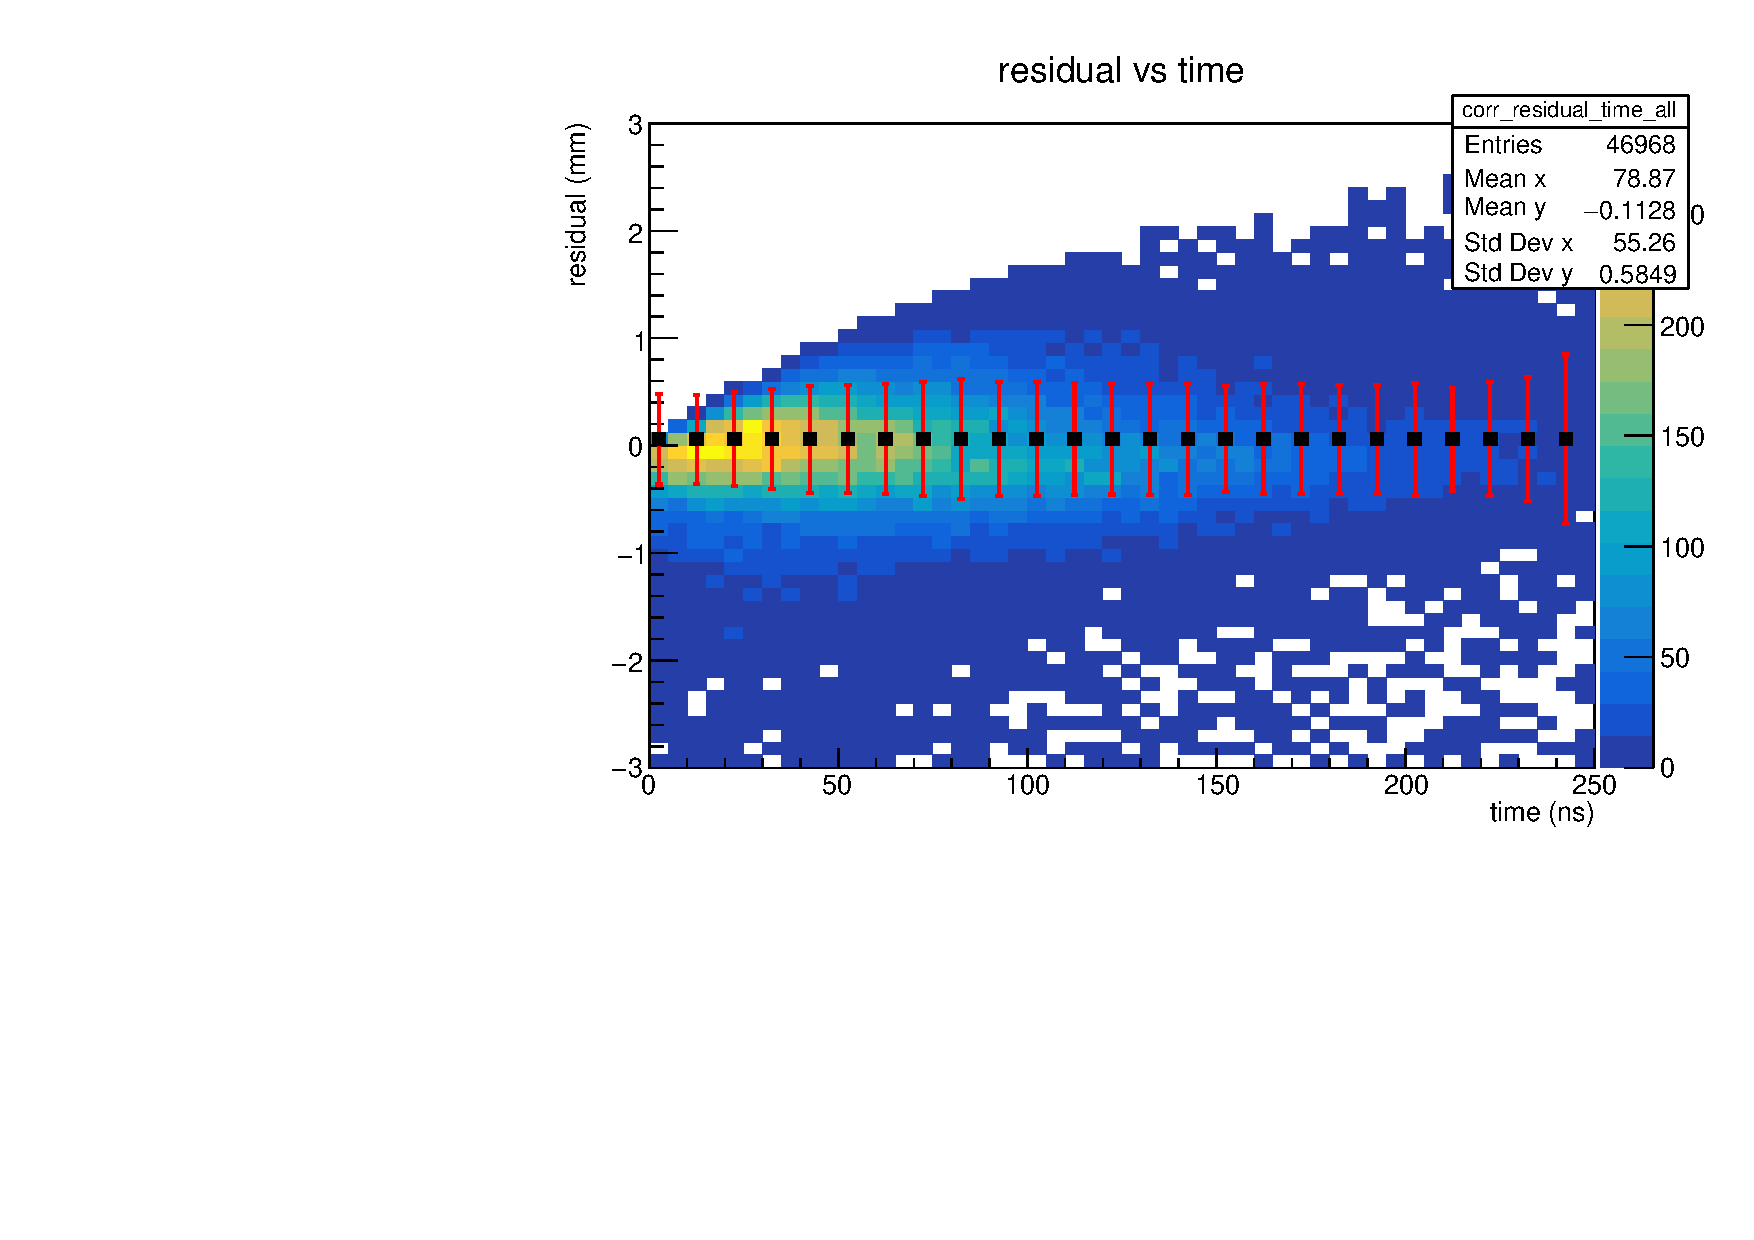
\includegraphics[width=\linewidth]{figures/residual_vs_time_2D.pdf}
        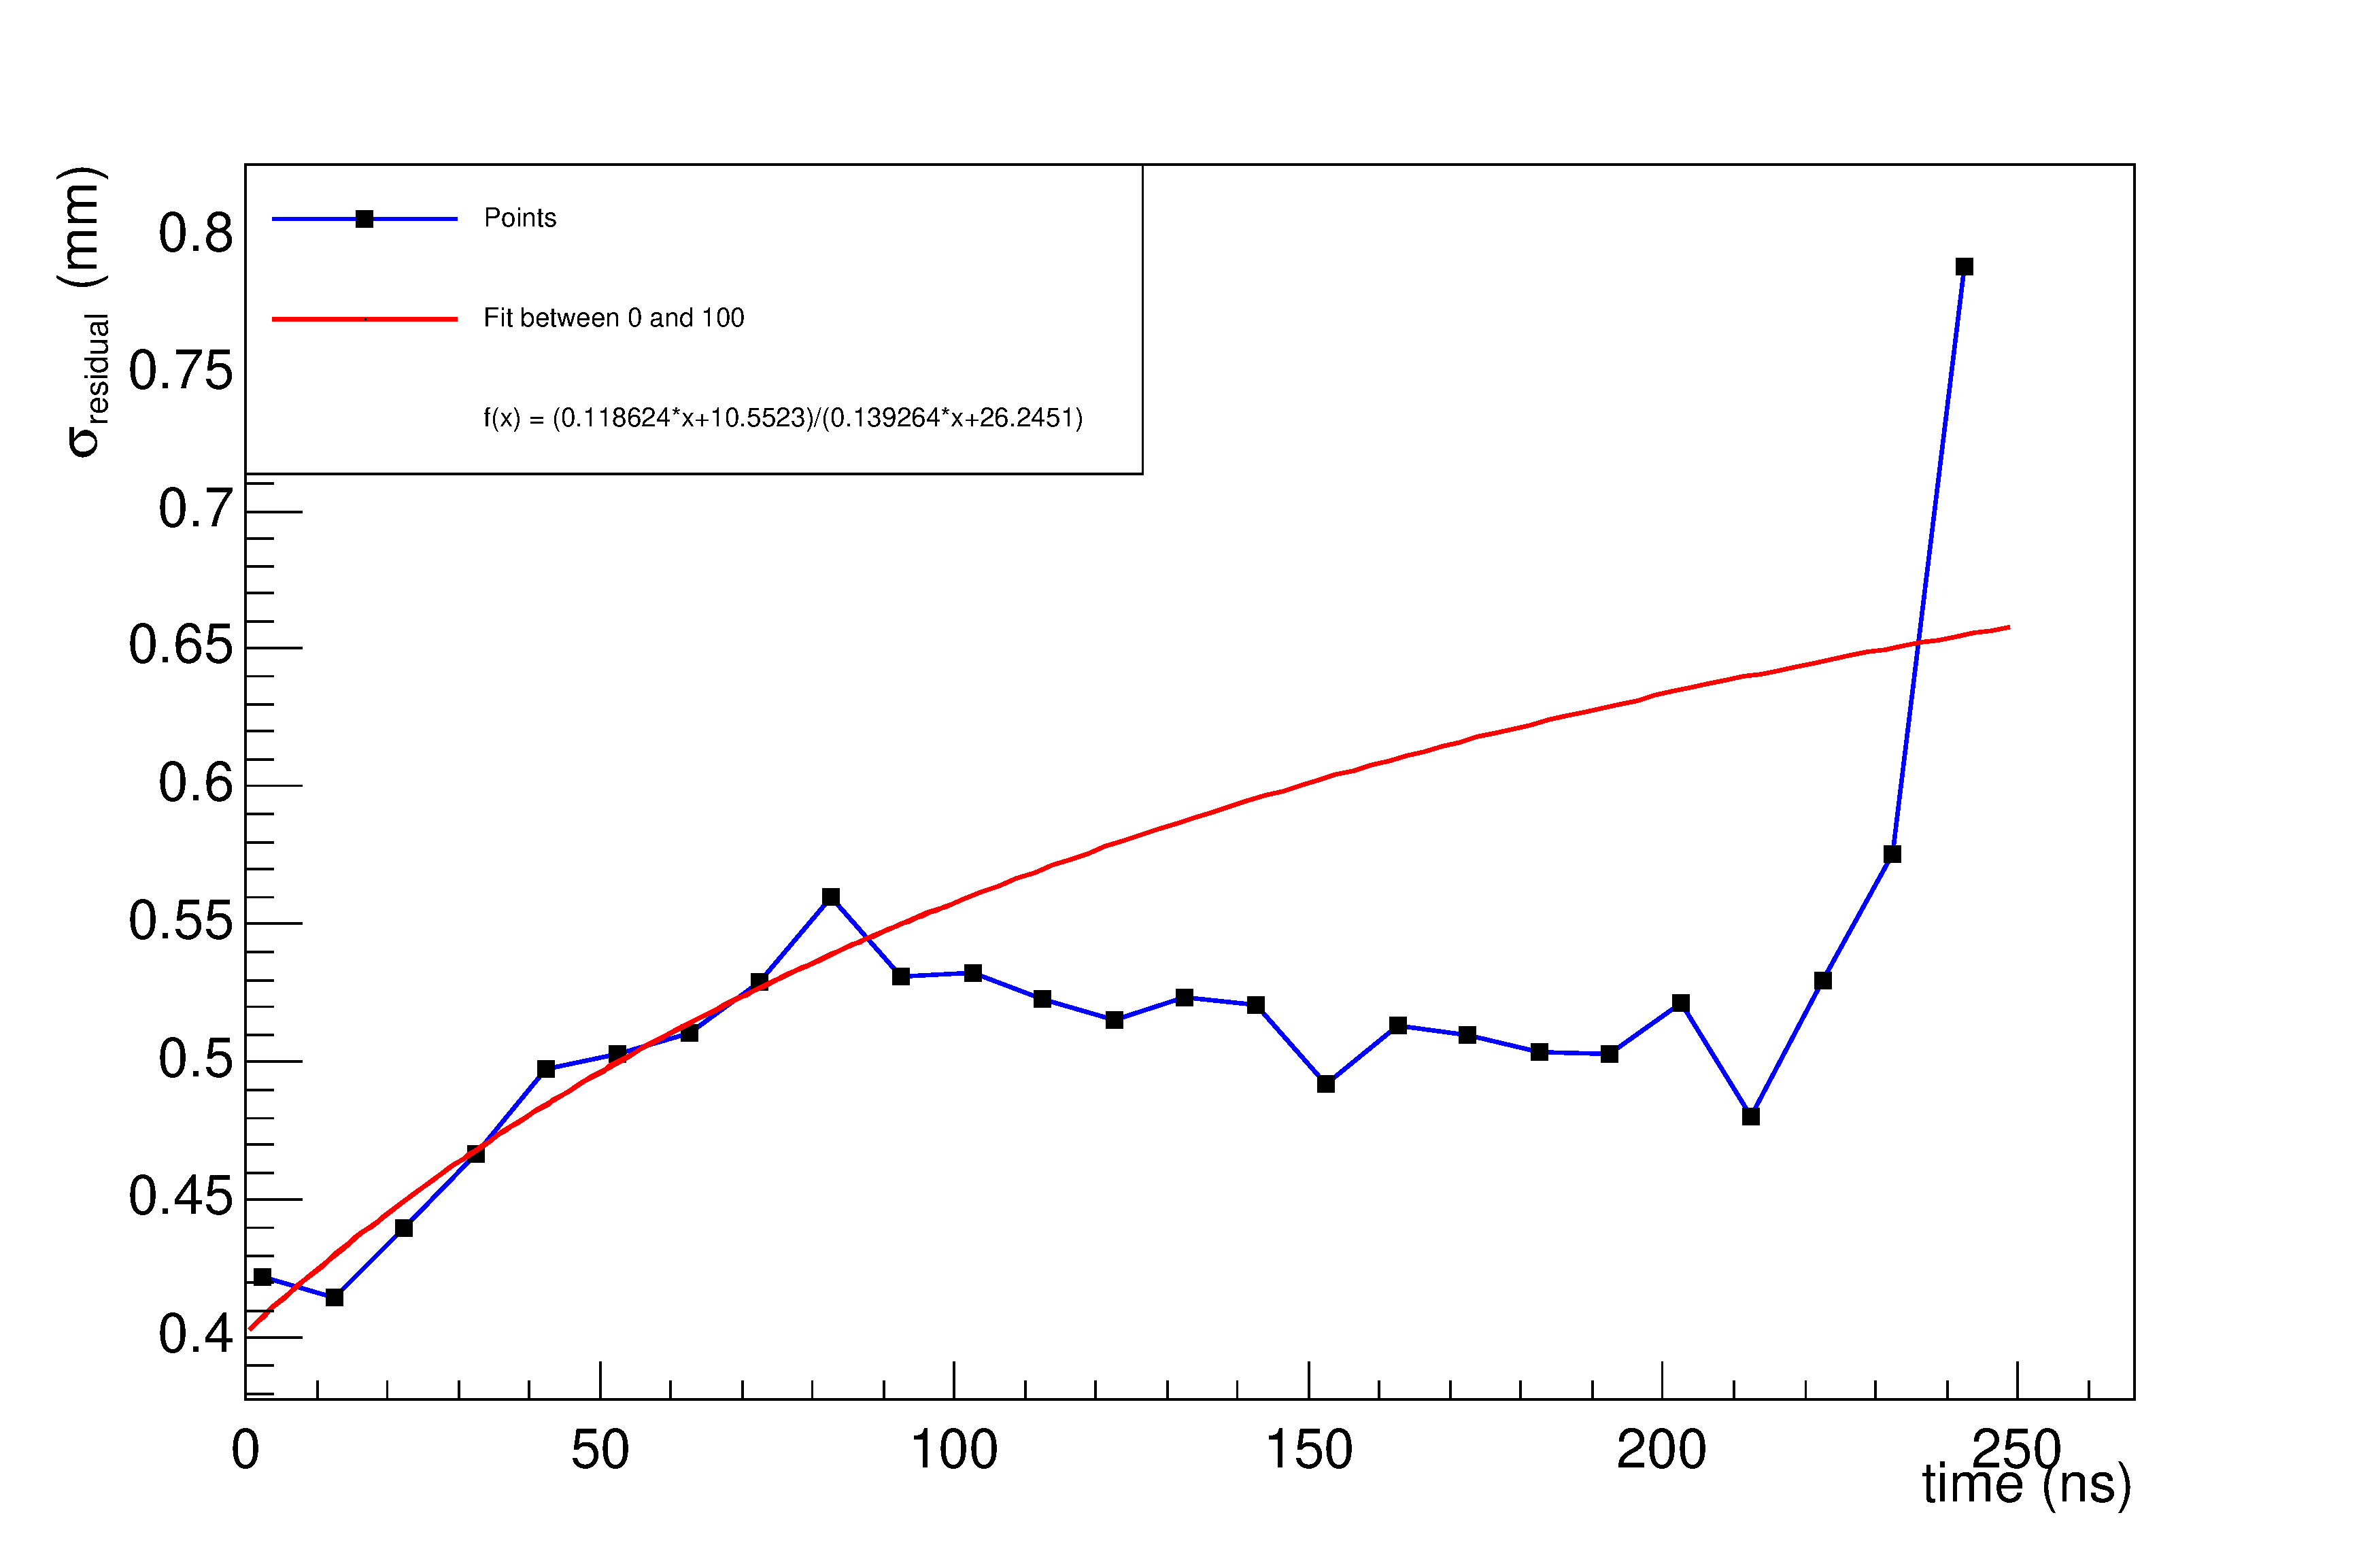
\includegraphics[width=\linewidth]{figures/resolution_residual_on_time.pdf}
    \end{minipage}

\end{frame}

\section{Implement the electron vertex}
\begin{frame}{Implement the electron vertex}
    \begin{itemize}
        \item The CLAS electron and the AHDC track comes from the same interaction point
        \item The electron vertex acts as an extra hit for the Kalman Filter
        \item The resolution in the beamline $\sigma_{r}^2$ and $\sigma_{z}^2$ may depend on $p_e$ and $\theta_e$
        \item For now we use constant values (0.09 mm$^2$ and 64 mm$^2$). A study will be done to give the expressions of $\sigma_{r}^2(p_e,\theta_e)$ and $\sigma_{z}^2(p_e,\theta_e)$.
    \end{itemize}

    \vspace{0.5cm}

    \centering
    \begin{minipage}{0.38\textwidth}
        \includegraphics[width=\linewidth]{figures/build/electron_vertex.pdf}
    \end{minipage}
    \hspace{0.5cm}
    \begin{minipage}{0.38\textwidth}
        - measurement:
        \[
            z = (0, \phi_{\mbox{\tiny arbitrary}}, v_{z_e})^T
        \]
        - error matrix:
        \[
        \begin{bmatrix}
            \sigma_{r}^2(p_e,\theta_e) & 0 & 0 \\
            0 & 1e10 & 0 \\
            0 & 0 & \sigma_{z}^2(p_e,\theta_e)
        \end{bmatrix}
        \]
    \end{minipage}

\end{frame}

\section{Make the Kalman Filter reusable}
\begin{frame}{Make the Kalman Filter reusable}
    \begin{itemize}
        \item We wanted to run the Kalman Filter at different stage of the tracking reconstruction
        \item For example, we knew that we would need to remove bad AHDC hits and/or use ATOF hits to improve the AHDC reconstruction
        \item Initially in the AHDCEngine, the Kalman Filter has been move to the ALERTEngine where it requires the ATOFEngine and the AHDCEngine to have run before
        \item It keeps track of the error covariance matrix from one use to another
    \end{itemize}

    \vspace{0.5cm}

\end{frame}

\section{Clean bad AHDC hits}
\begin{frame}{Clean bad AHDC hits}
    \begin{itemize}
        \item When the AHDC occupancy is big, some noisy hit can be associated to a track (e.g n $\ge$ 2 hits on the same layer); but now the Kalman Filter consider every hit.
        \item To fix it:
            \begin{itemize}
                \item We run the Kalman Filter (KF1) $\rightarrow$ the residuals of all hits are accessible
                \item We remove the hits for which the residuals are very big (e.g. $\ge 1.5$ mm)
                \item We rerun the Kalman Filter on the remaining hits (KF2) with less Niter
            \end{itemize}
        \item These are distributions for elastic events from run 22712.

    \end{itemize}

    \vspace{0.5cm}

    \centering
    \begin{minipage}{0.42\textwidth}
        \begin{tikzpicture}
            \node[anchor=south west, inner sep=0] (image) at (0,0) {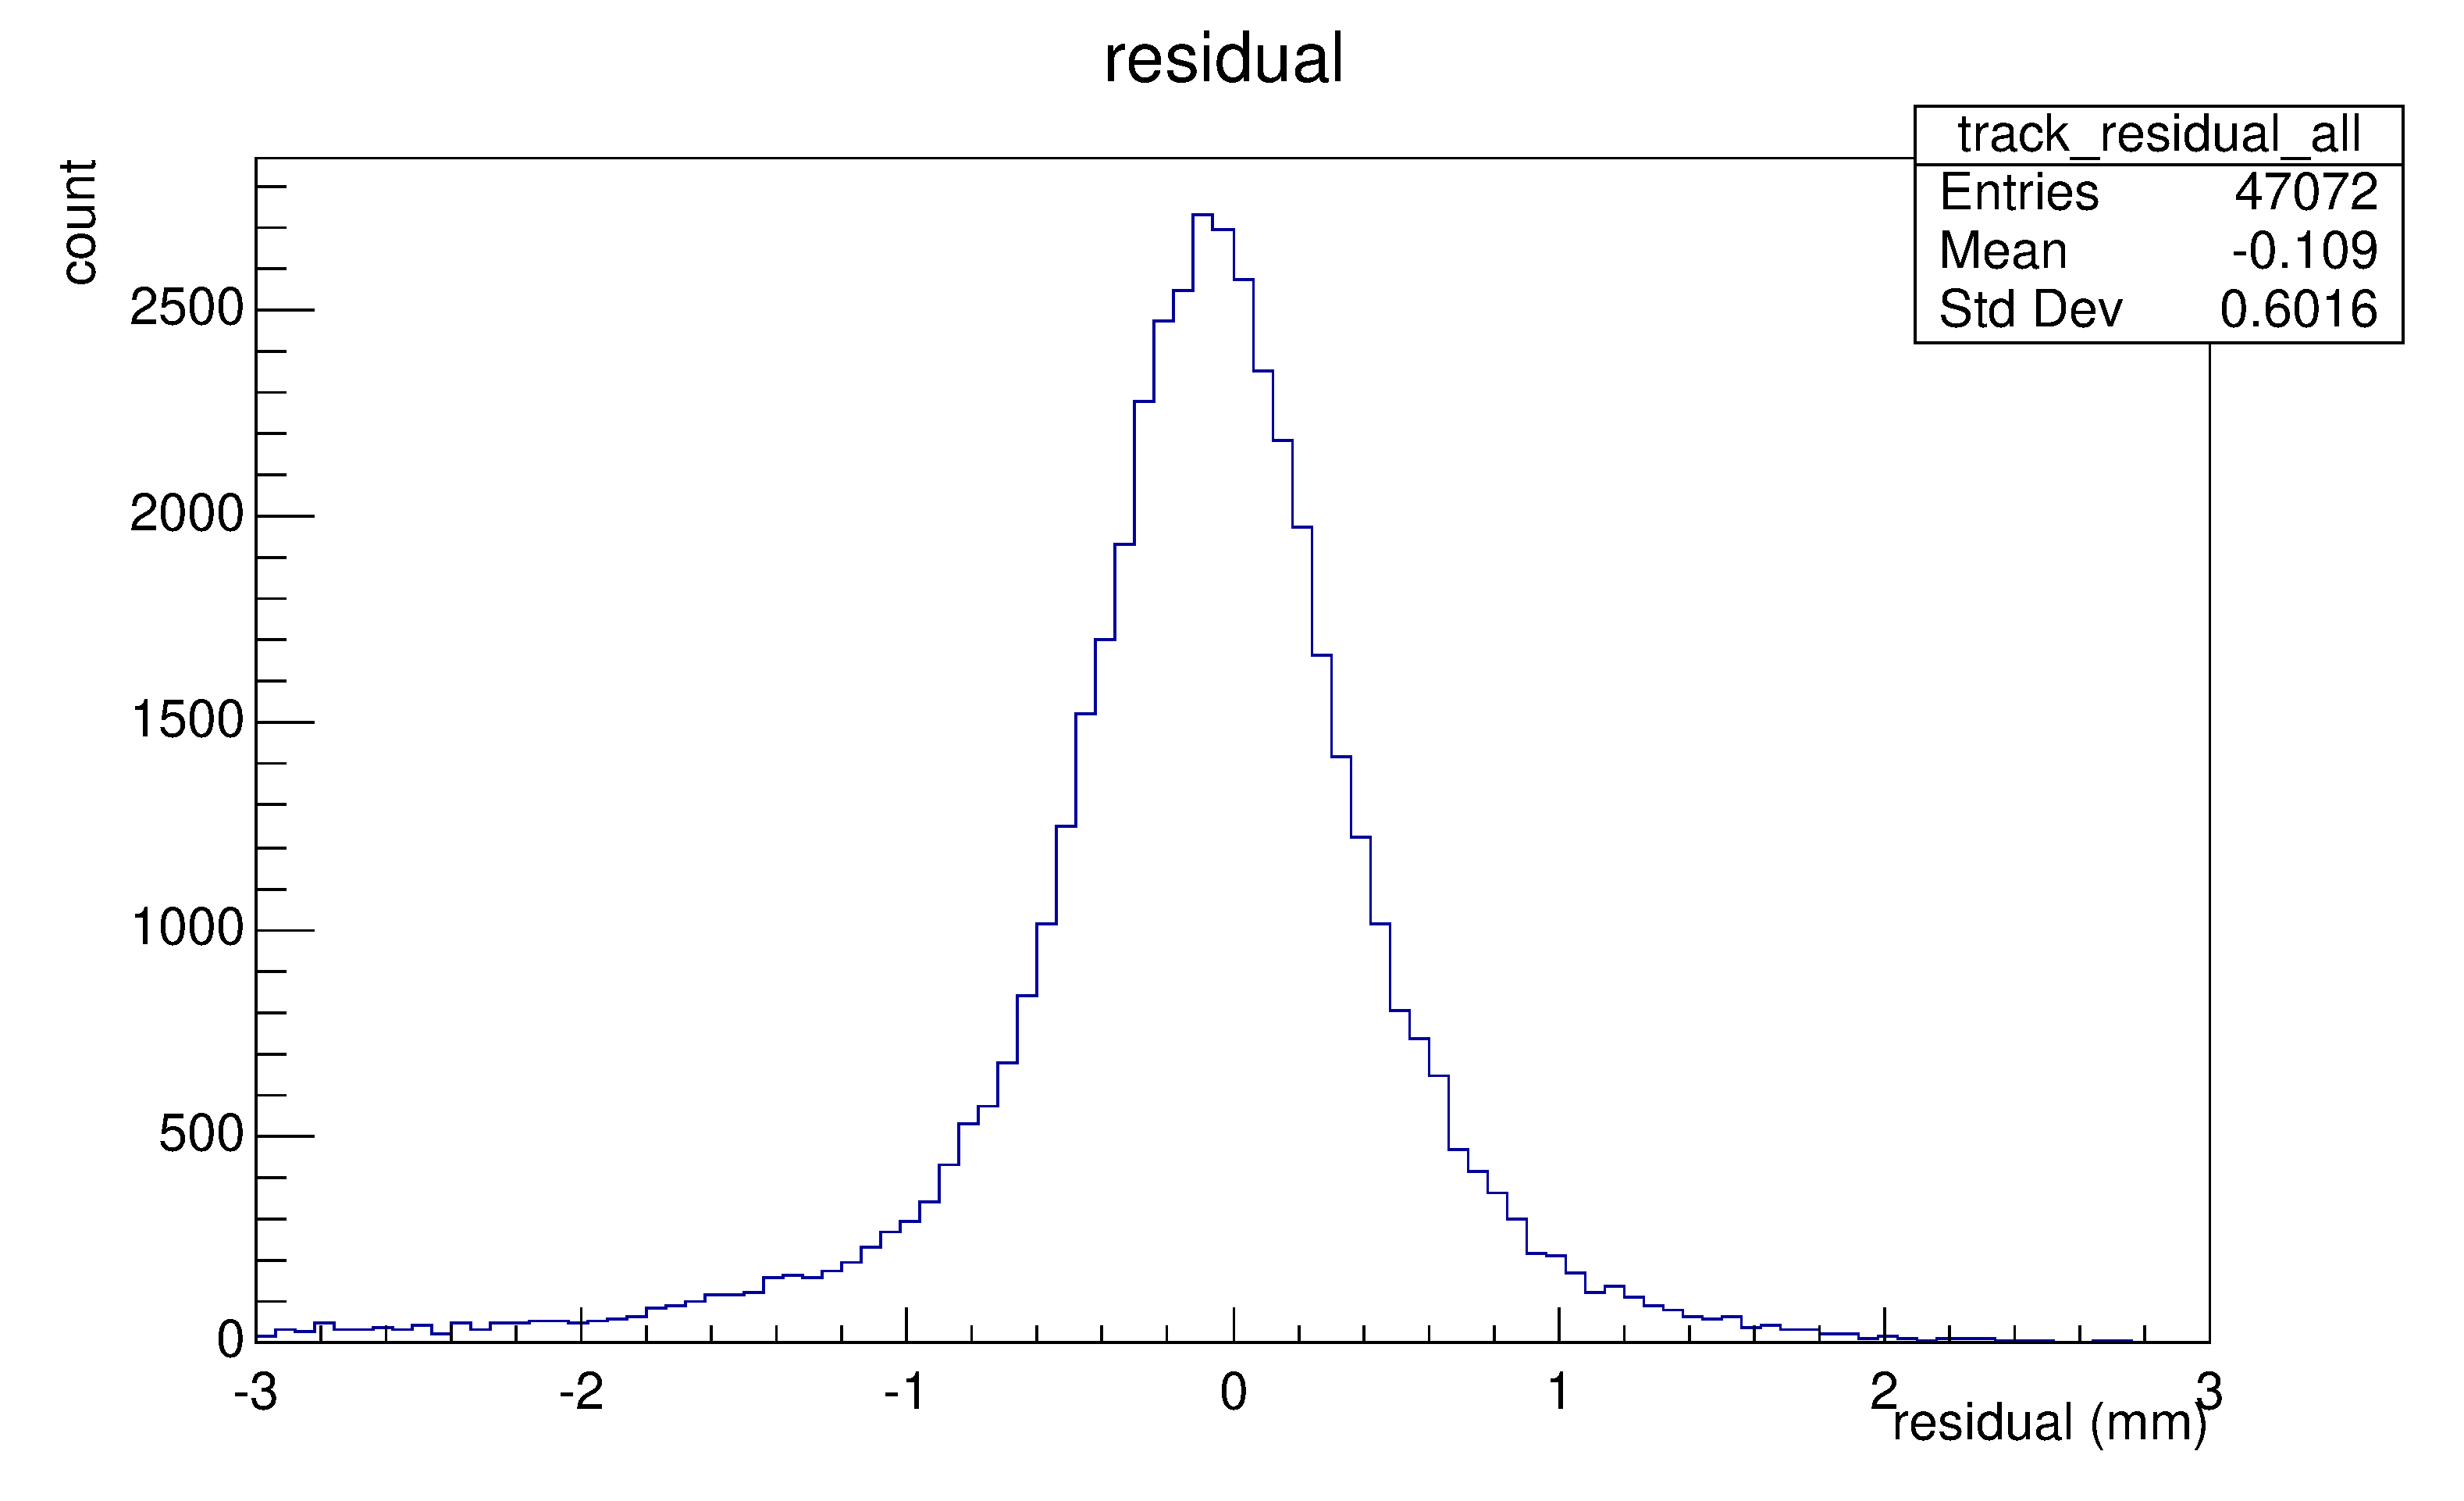
\includegraphics[width=\linewidth]{figures/residual_before_hit_cleaning_real_data.pdf}};
            % Option : système de coordonnées relatif (0 à 1)
            \begin{scope}[x={(image.south east)}, y={(image.north west)}]
                \node [red] at (0.7,0.6) {\tiny before};
            \end{scope}
        \end{tikzpicture}
    \end{minipage}
    \begin{minipage}{0.42\textwidth}
        \begin{tikzpicture}
            \node[anchor=south west, inner sep=0] (image) at (0,0) {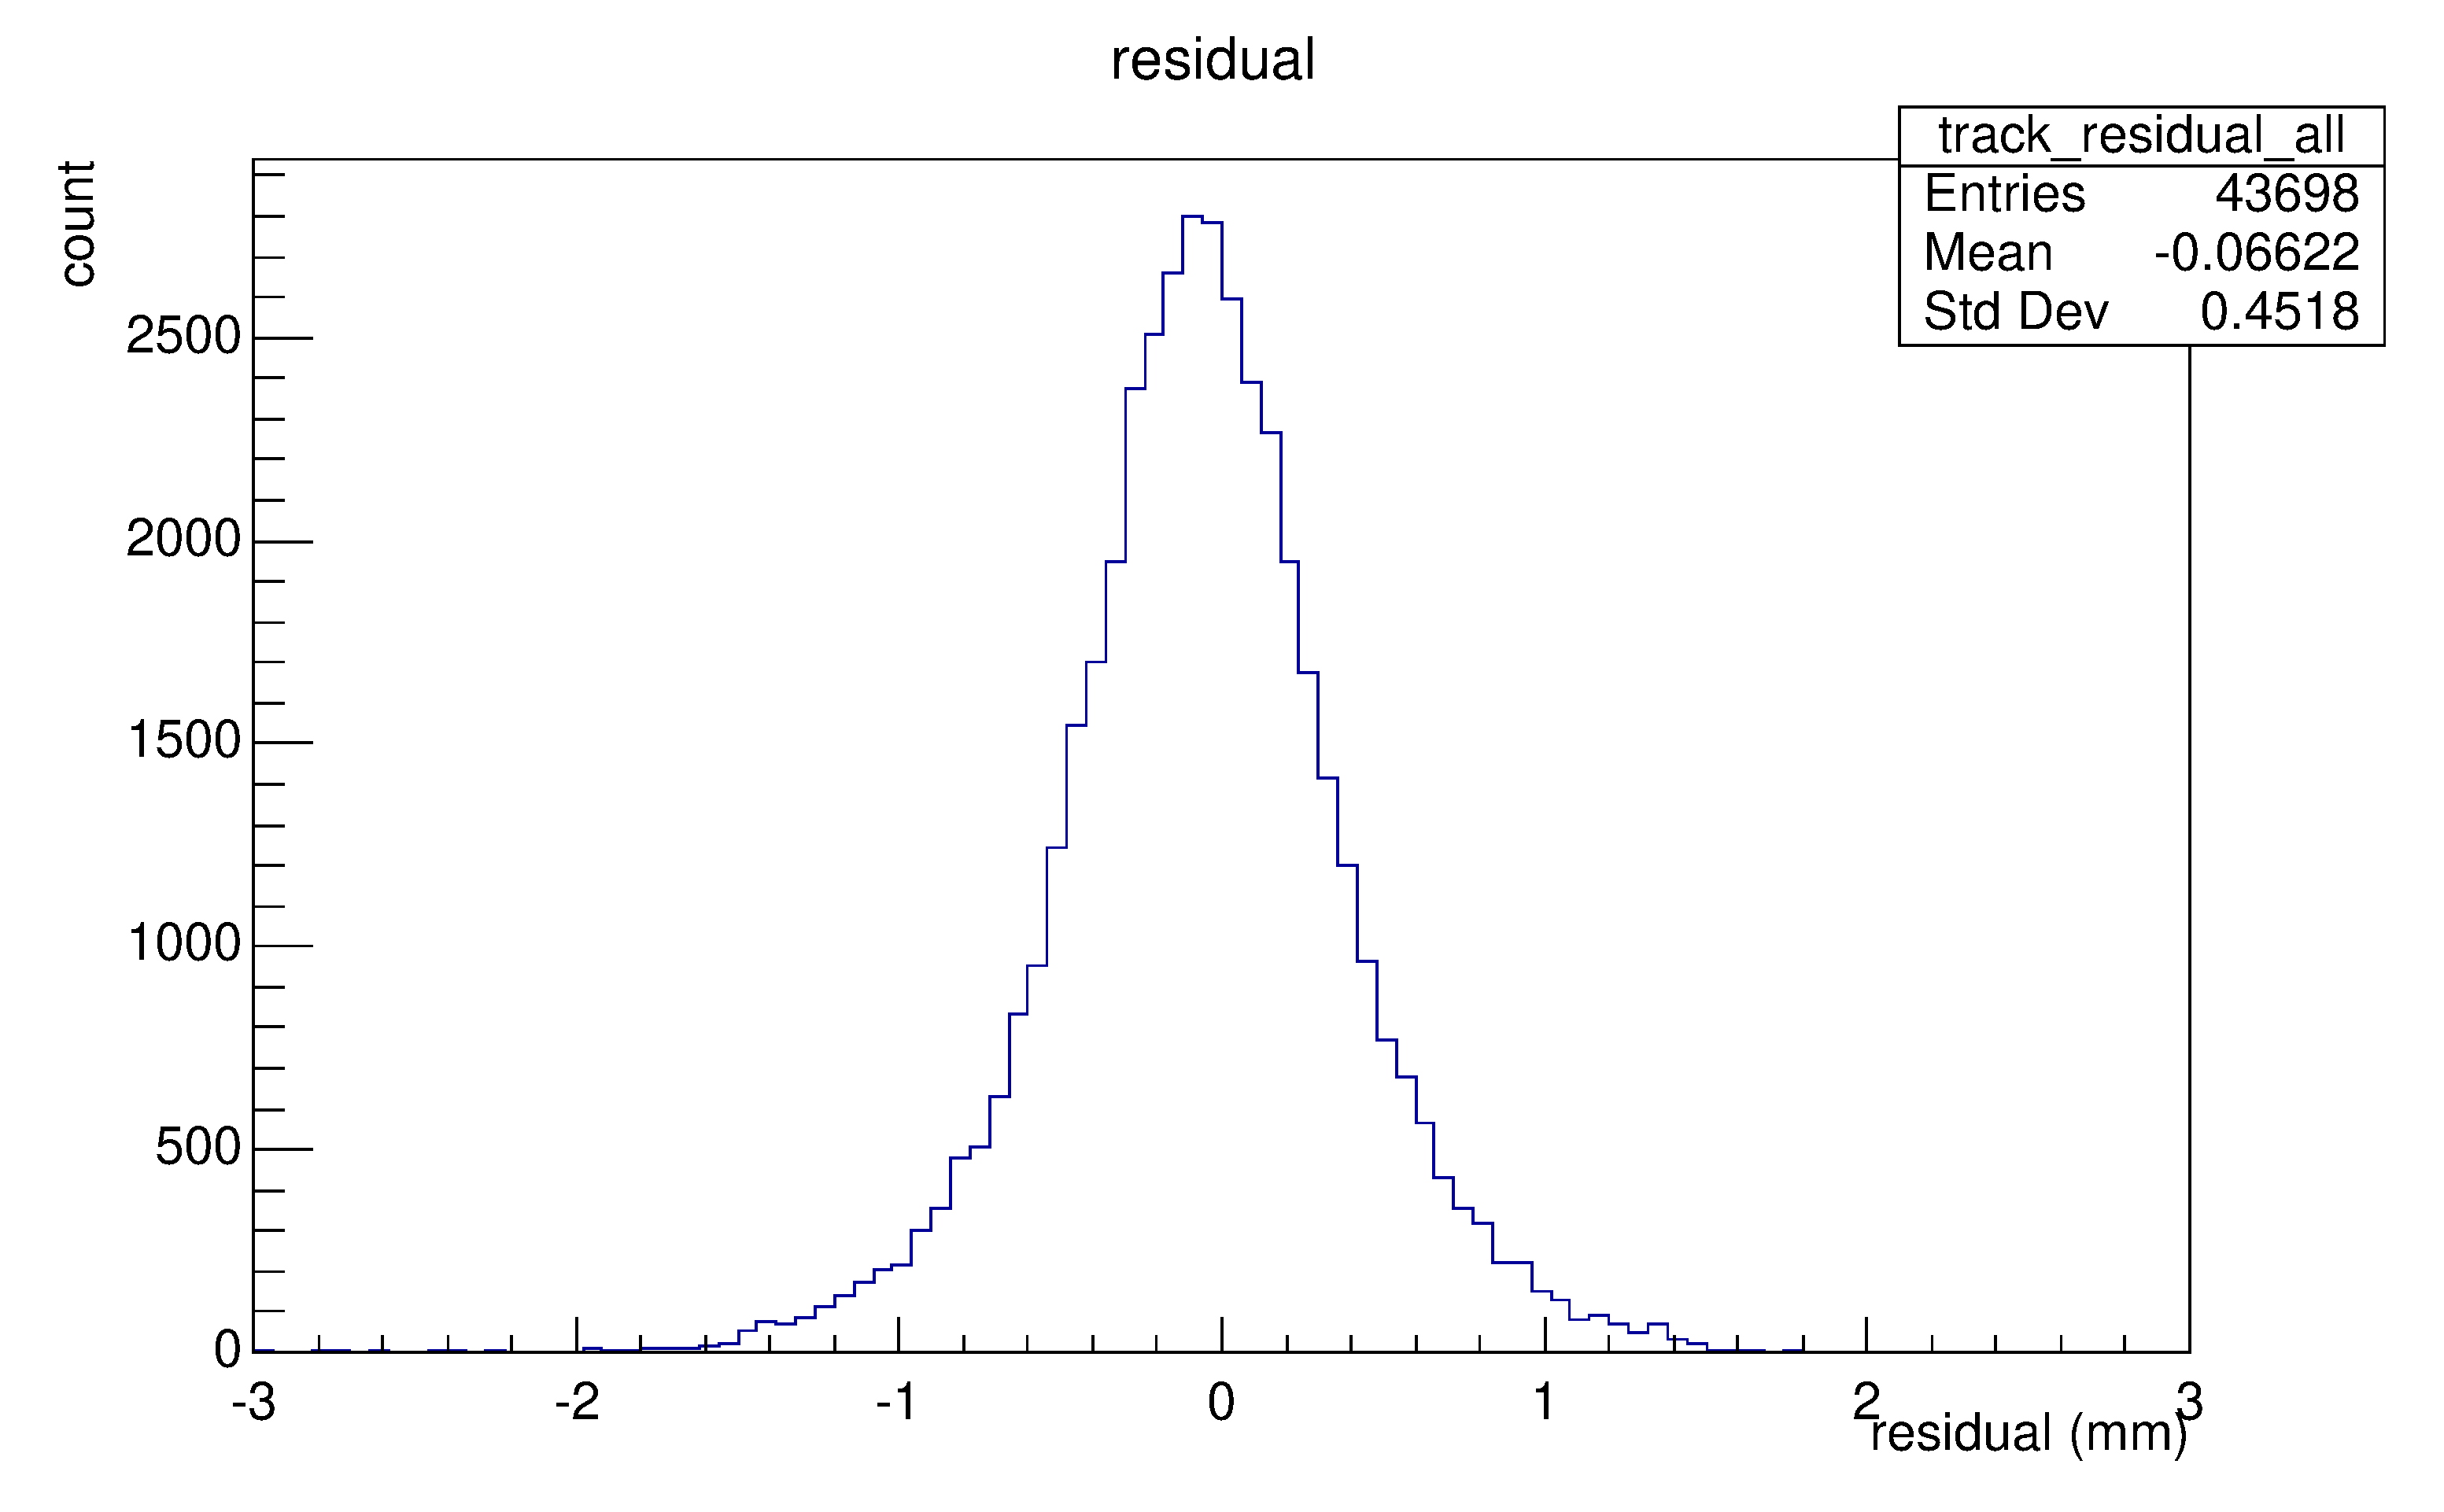
\includegraphics[width=\linewidth]{figures/residual_after_hit_cleaning_real_data.pdf}};
            % Option : système de coordonnées relatif (0 à 1)
            \begin{scope}[x={(image.south east)}, y={(image.north west)}]
                \node [red] at (0.7,0.6) {\tiny after};
            \end{scope}
        \end{tikzpicture}
    \end{minipage}

\end{frame}

\section{AHDC geometry issue}
\begin{frame}{AHDC geometry issue 1/2}
    \begin{itemize}
        \item We noticed that the theta reconstruction was much better in simulation compared to real data
        \item We found that the geometry encoded in coatjava differed from the final designed of the detector
    \end{itemize}

    \vspace{0.3cm}

    \centering
    \begin{minipage}{0.4\textwidth}
        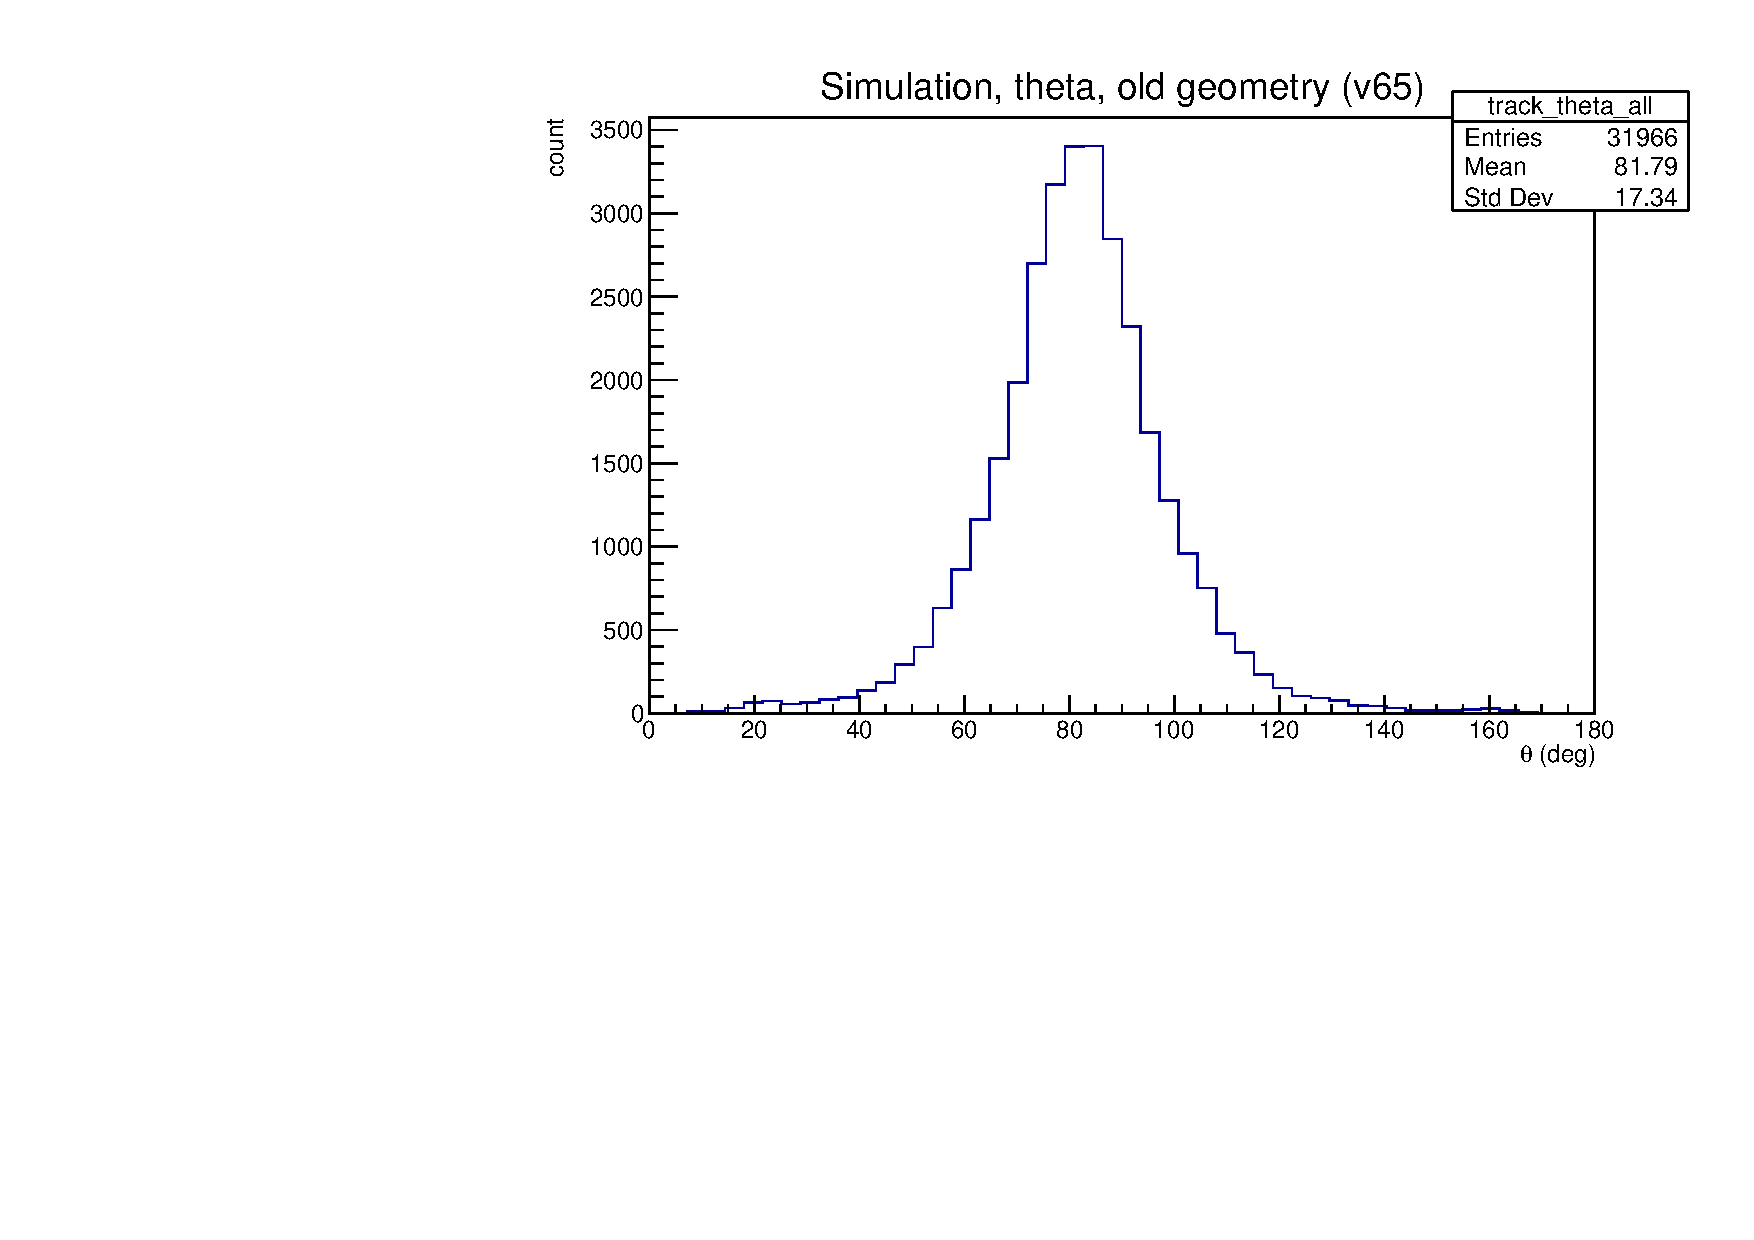
\includegraphics[width=\linewidth]{figures/simu_theta_old_geometry.pdf}
        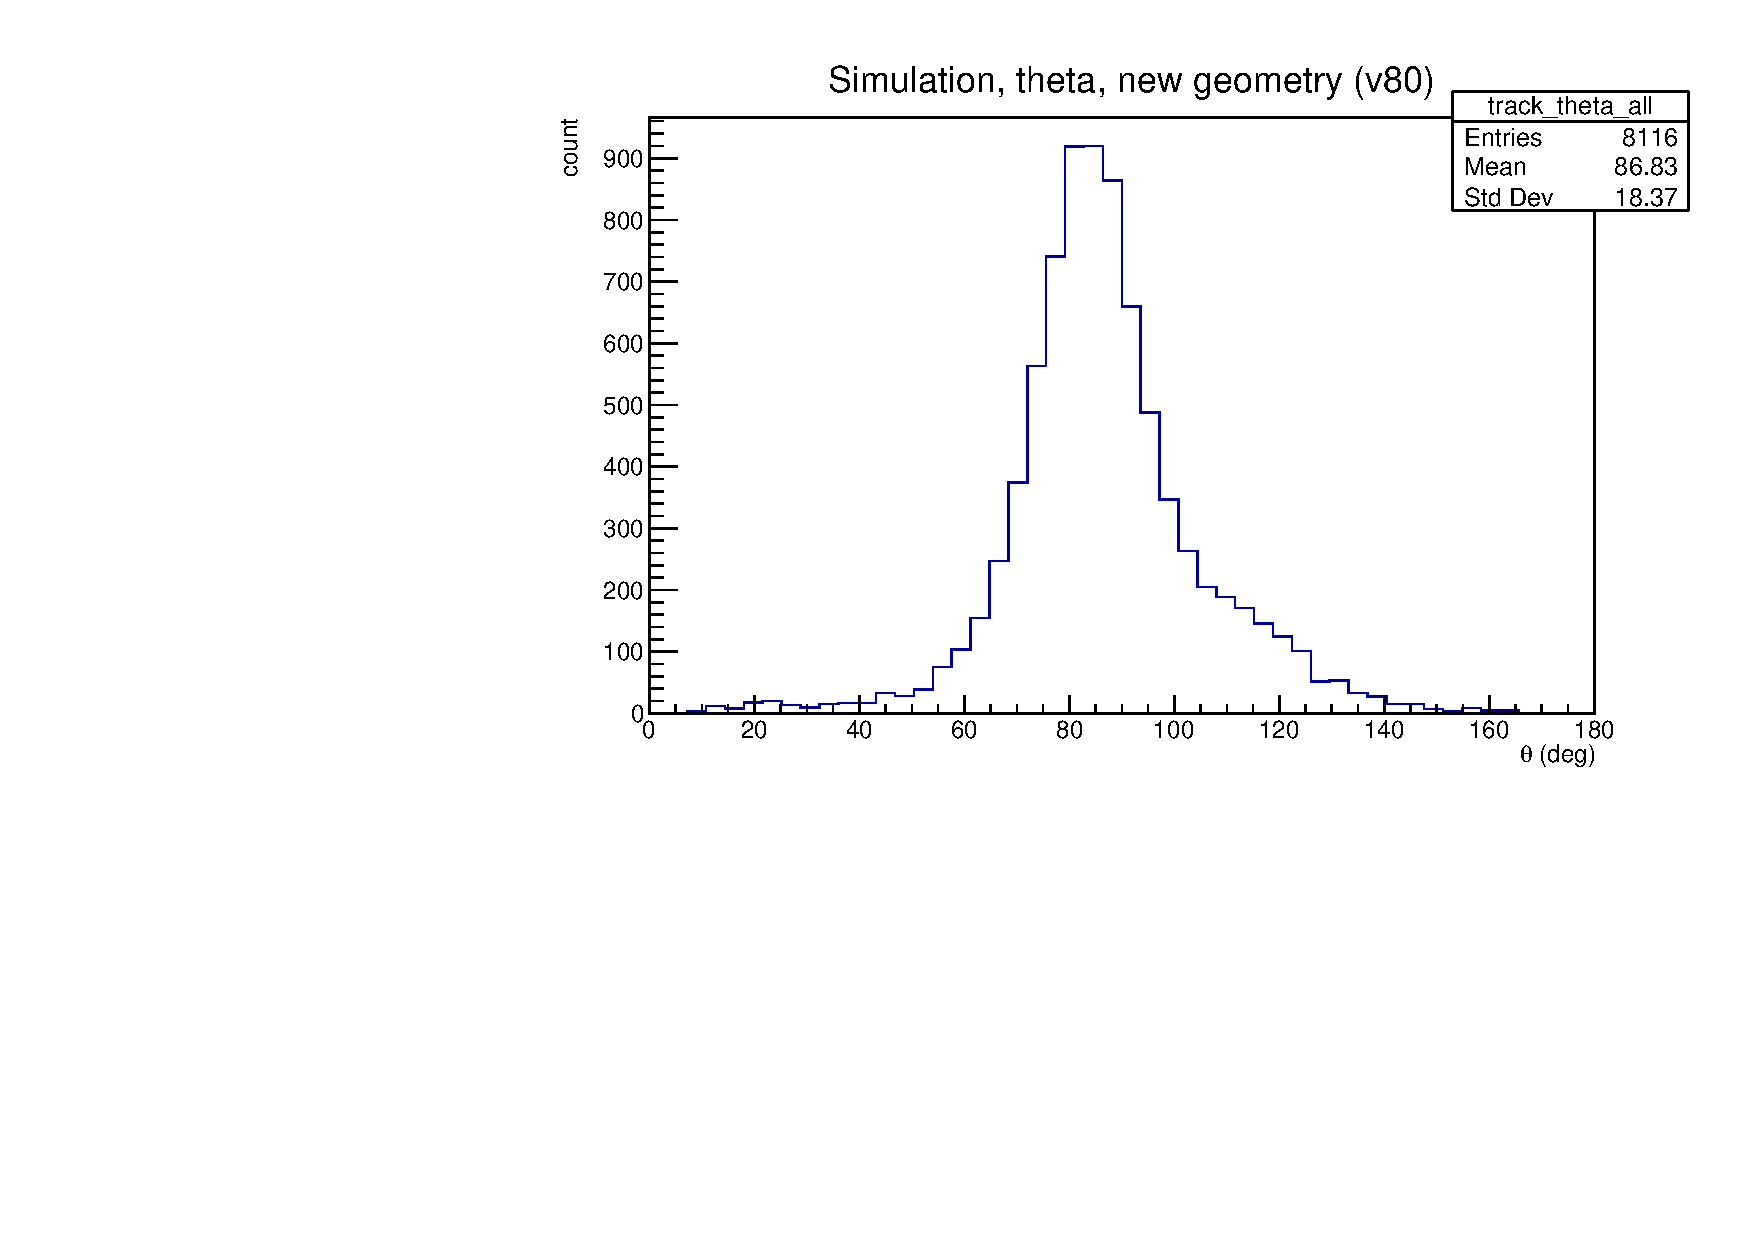
\includegraphics[width=\linewidth]{figures/simu_theta_new_geometry.pdf}
    \end{minipage}
    \begin{minipage}{0.4\textwidth}
        \begin{tikzpicture}
            \node[anchor=south west, inner sep=0] (image) at (0,0) {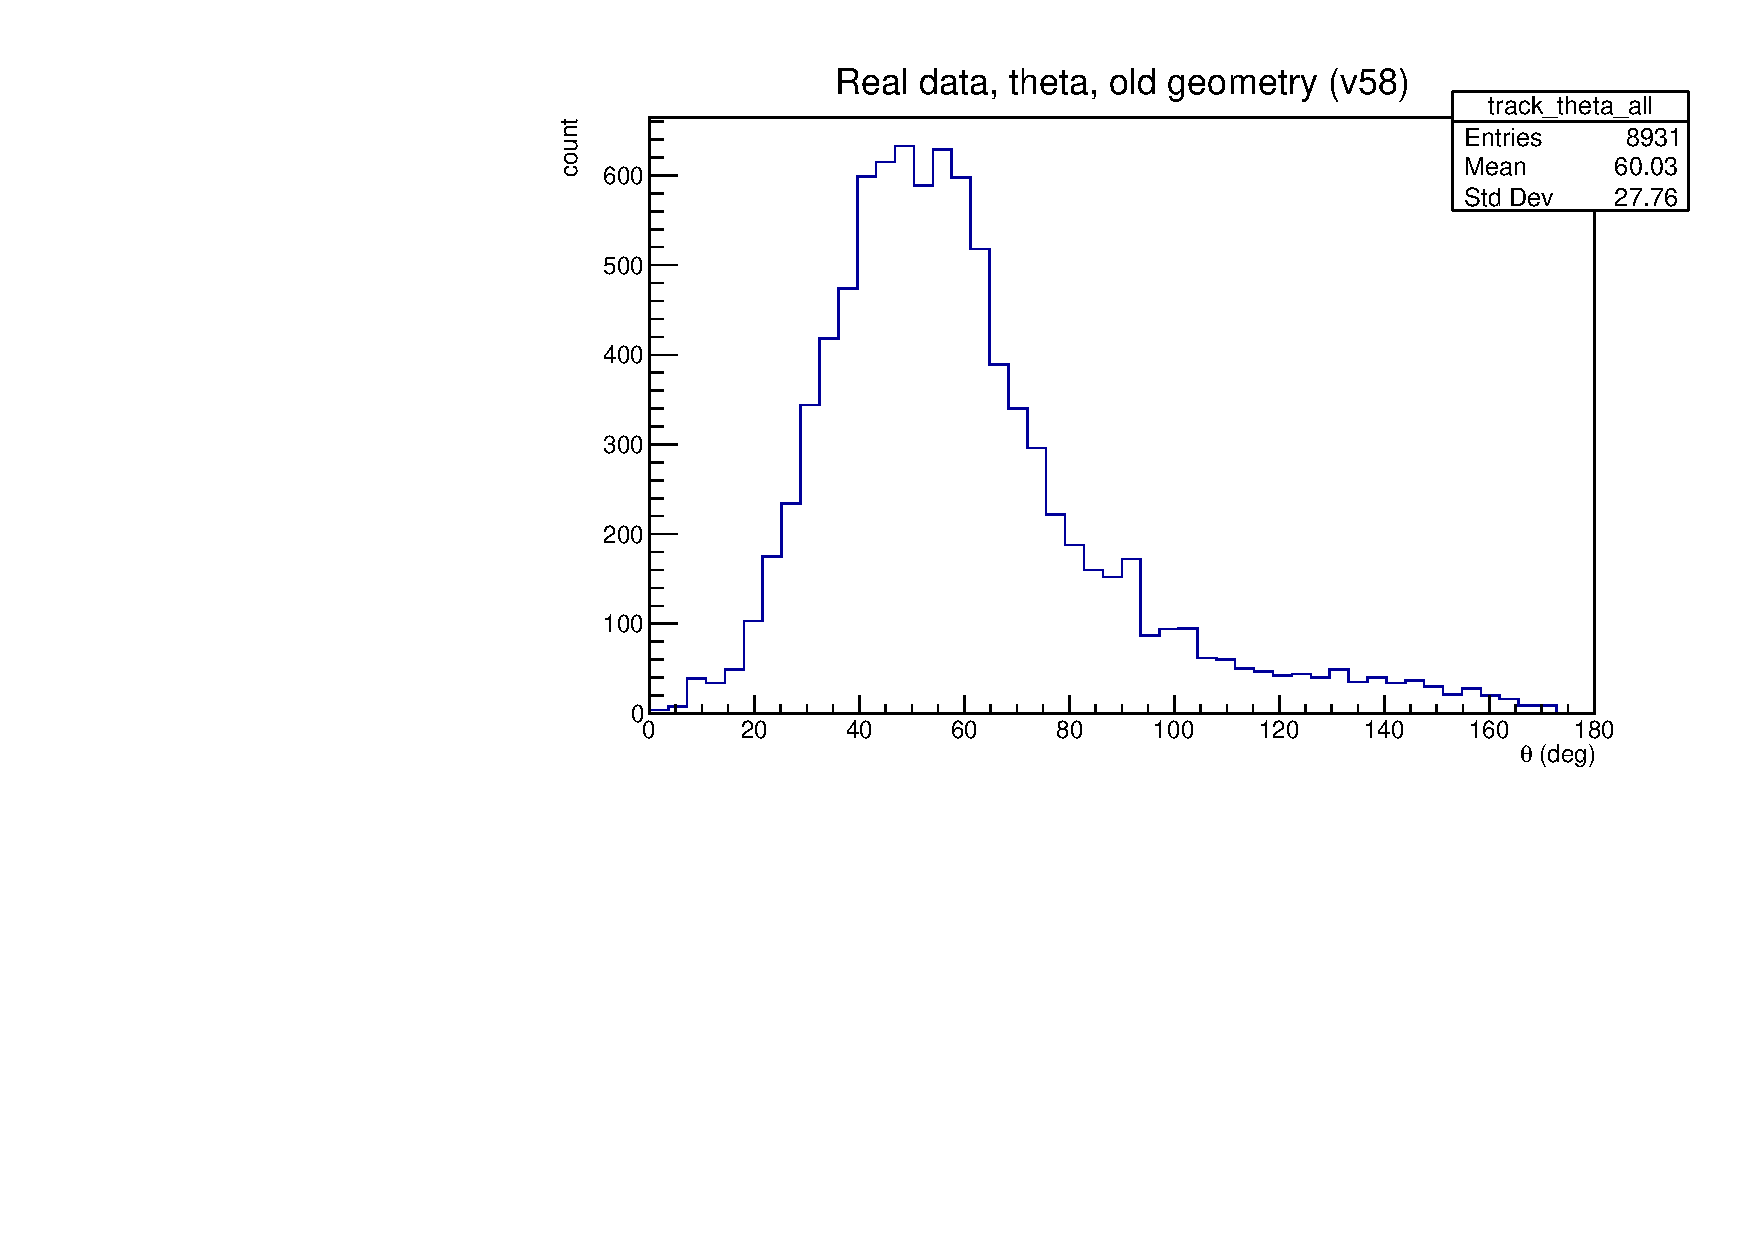
\includegraphics[width=\linewidth]{figures/data_theta_old_geometry.pdf}};
            % Option : système de coordonnées relatif (0 à 1)
            \begin{scope}[x={(image.south east)}, y={(image.north west)}]
                \node [red] at (0.7,0.6) {\tiny before};
            \end{scope}
        \end{tikzpicture}
        \begin{tikzpicture}
            \node[anchor=south west, inner sep=0] (image) at (0,0) {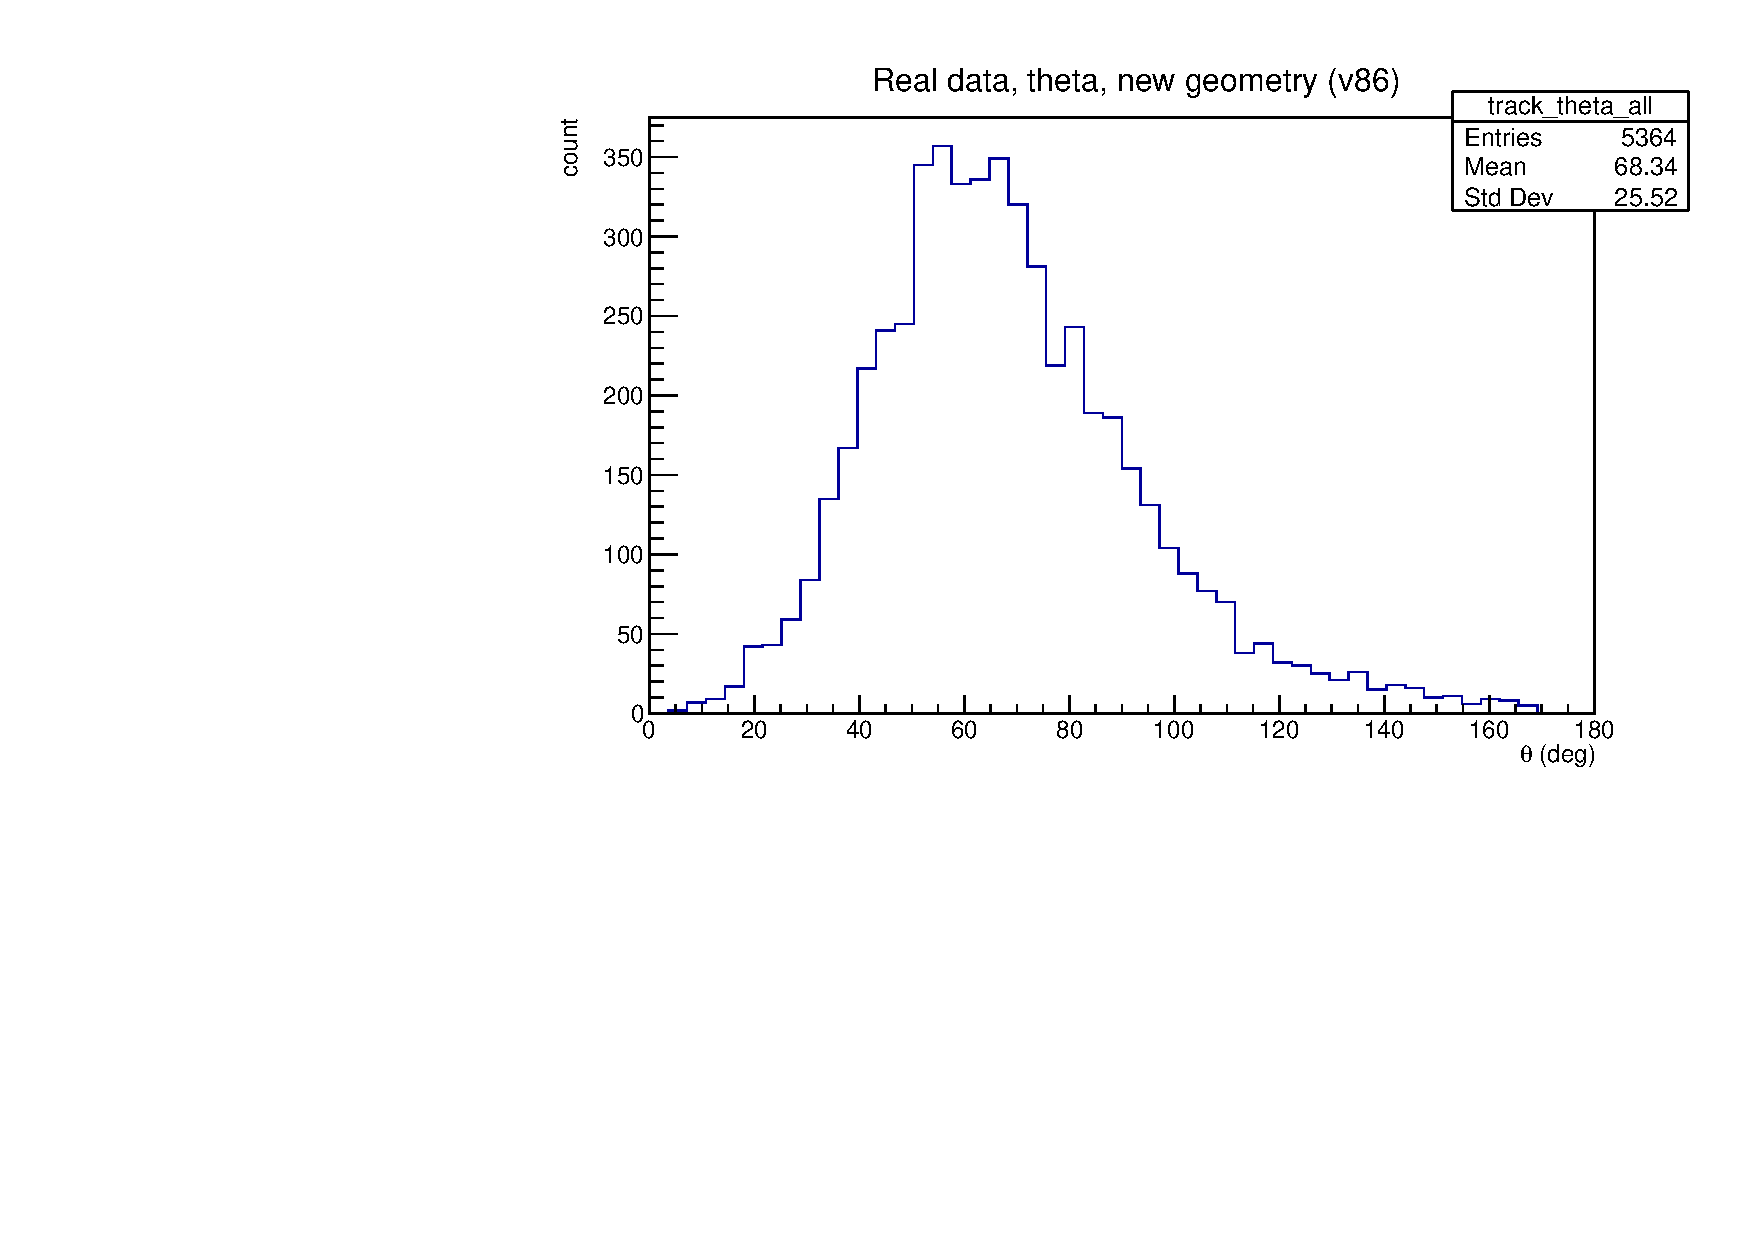
\includegraphics[width=\linewidth]{figures/data_theta_new_geometry.pdf}};
            % Option : système de coordonnées relatif (0 à 1)
            \begin{scope}[x={(image.south east)}, y={(image.north west)}]
                \node [red] at (0.7,0.6) {\tiny after};
            \end{scope}
        \end{tikzpicture}
    \end{minipage}

\end{frame}

\begin{frame}{AHDC geometry issue 2/2}
    \begin{itemize}
        \item Indeed, the end points of the detector are -188 mm and +162 mm instead of $\pm$150 mm on the z axis. The stereo angles are not exactly 20$^\circ$ but: 19.1489$^\circ$, 19.2857$^\circ$, 20.0$^\circ$, 20.6897$^\circ$, 20.0$^\circ$ respectively for each super layer
        \item We saw a small improvement, but still, we were far from the expect value
    \end{itemize}

    % A small improvement in the sense that wez shift to the right direction.

    \vspace{0.3cm}

    \centering
    \begin{minipage}{0.4\textwidth}
        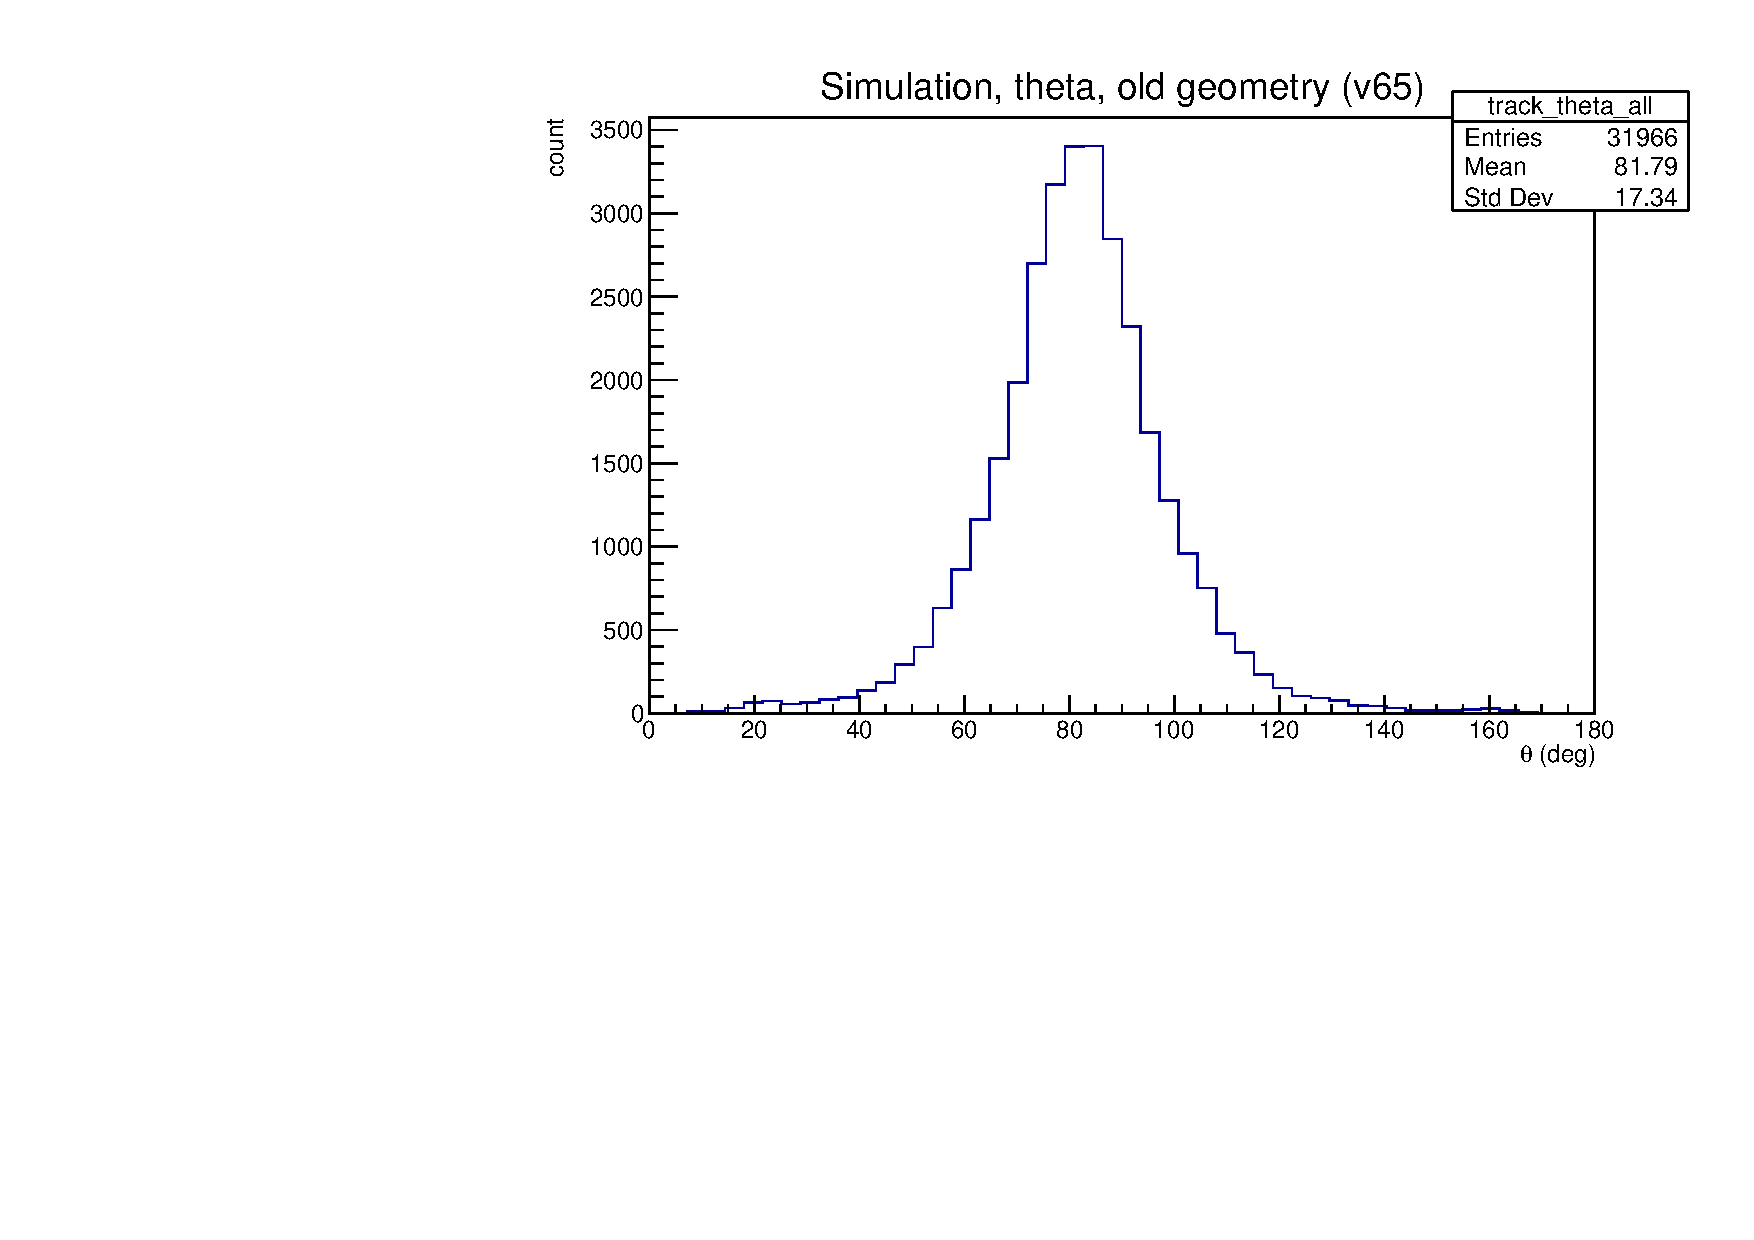
\includegraphics[width=\linewidth]{figures/simu_theta_old_geometry.pdf}
        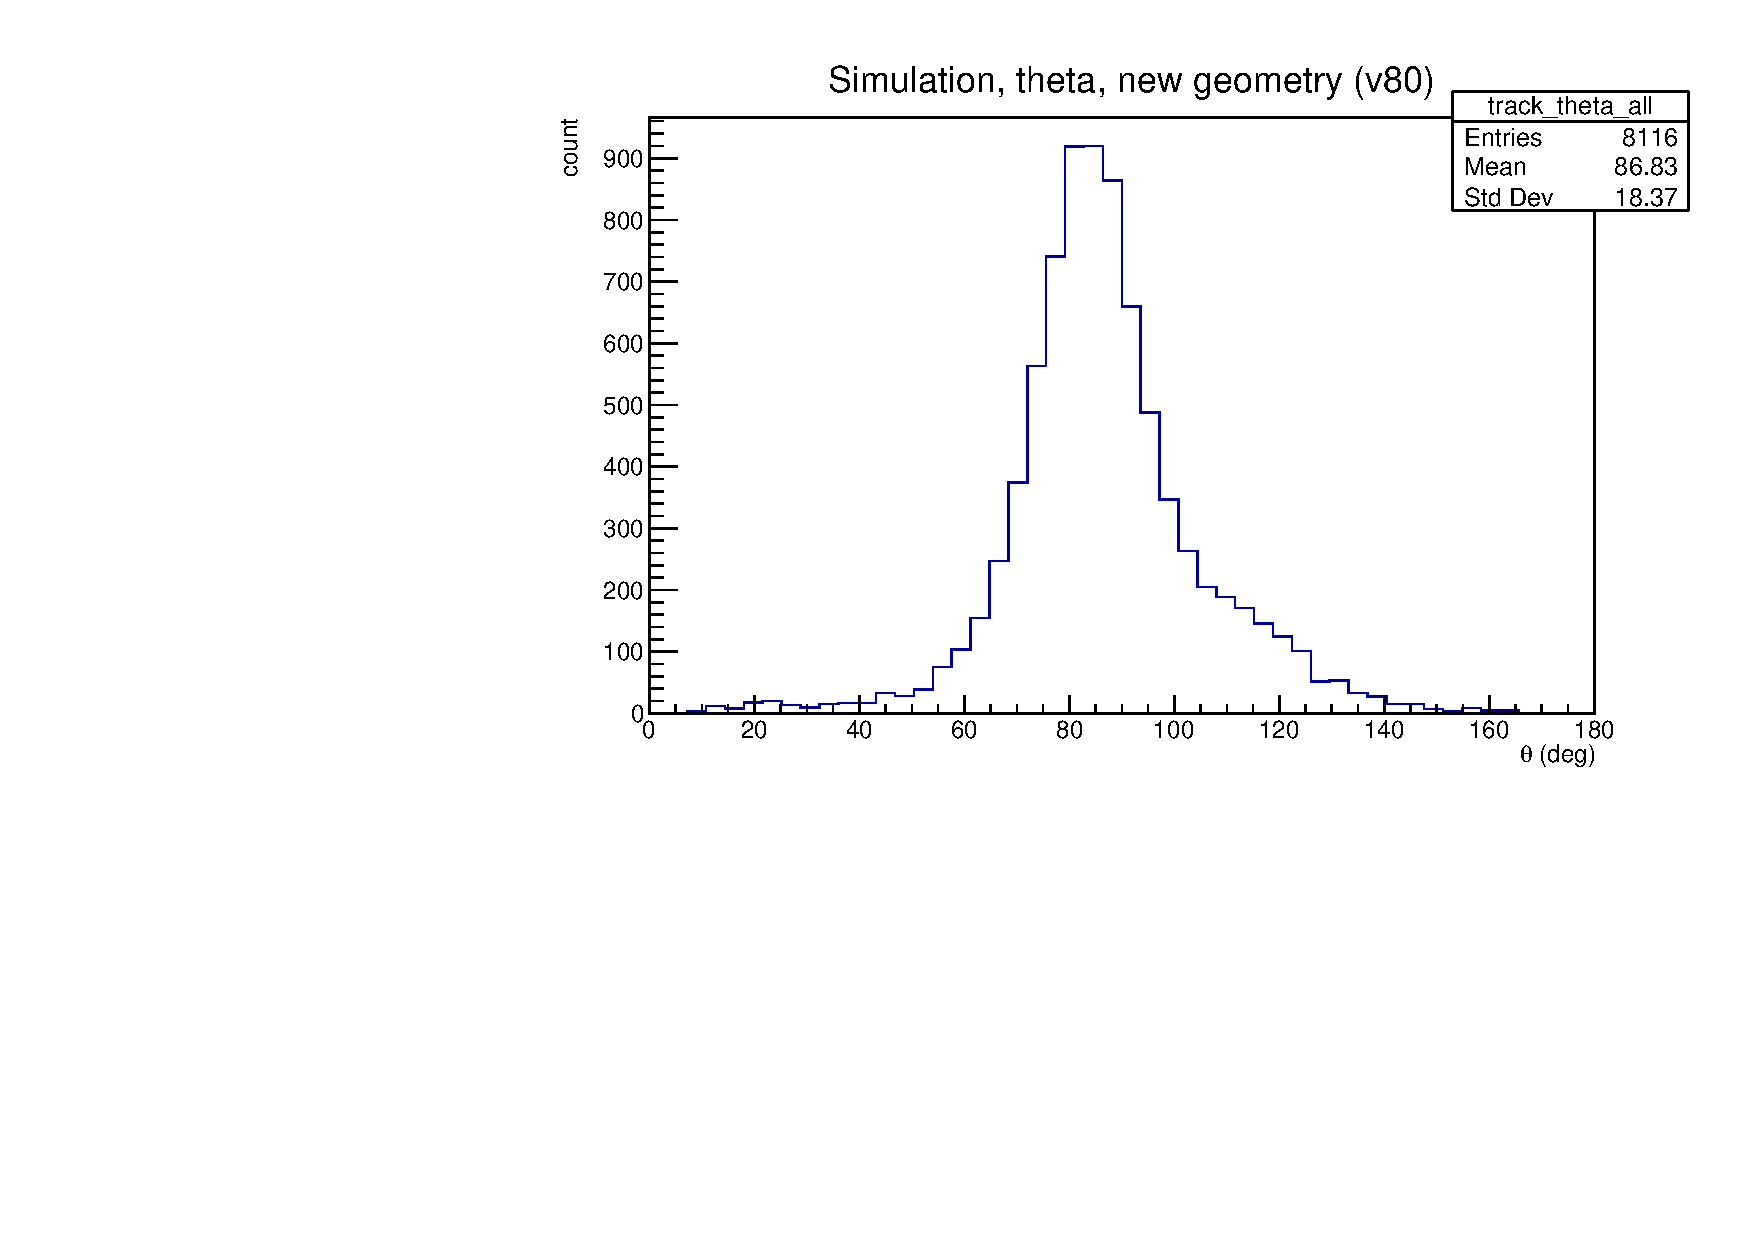
\includegraphics[width=\linewidth]{figures/simu_theta_new_geometry.pdf}
    \end{minipage}
    \begin{minipage}{0.4\textwidth}
        \begin{tikzpicture}
            \node[anchor=south west, inner sep=0] (image) at (0,0) {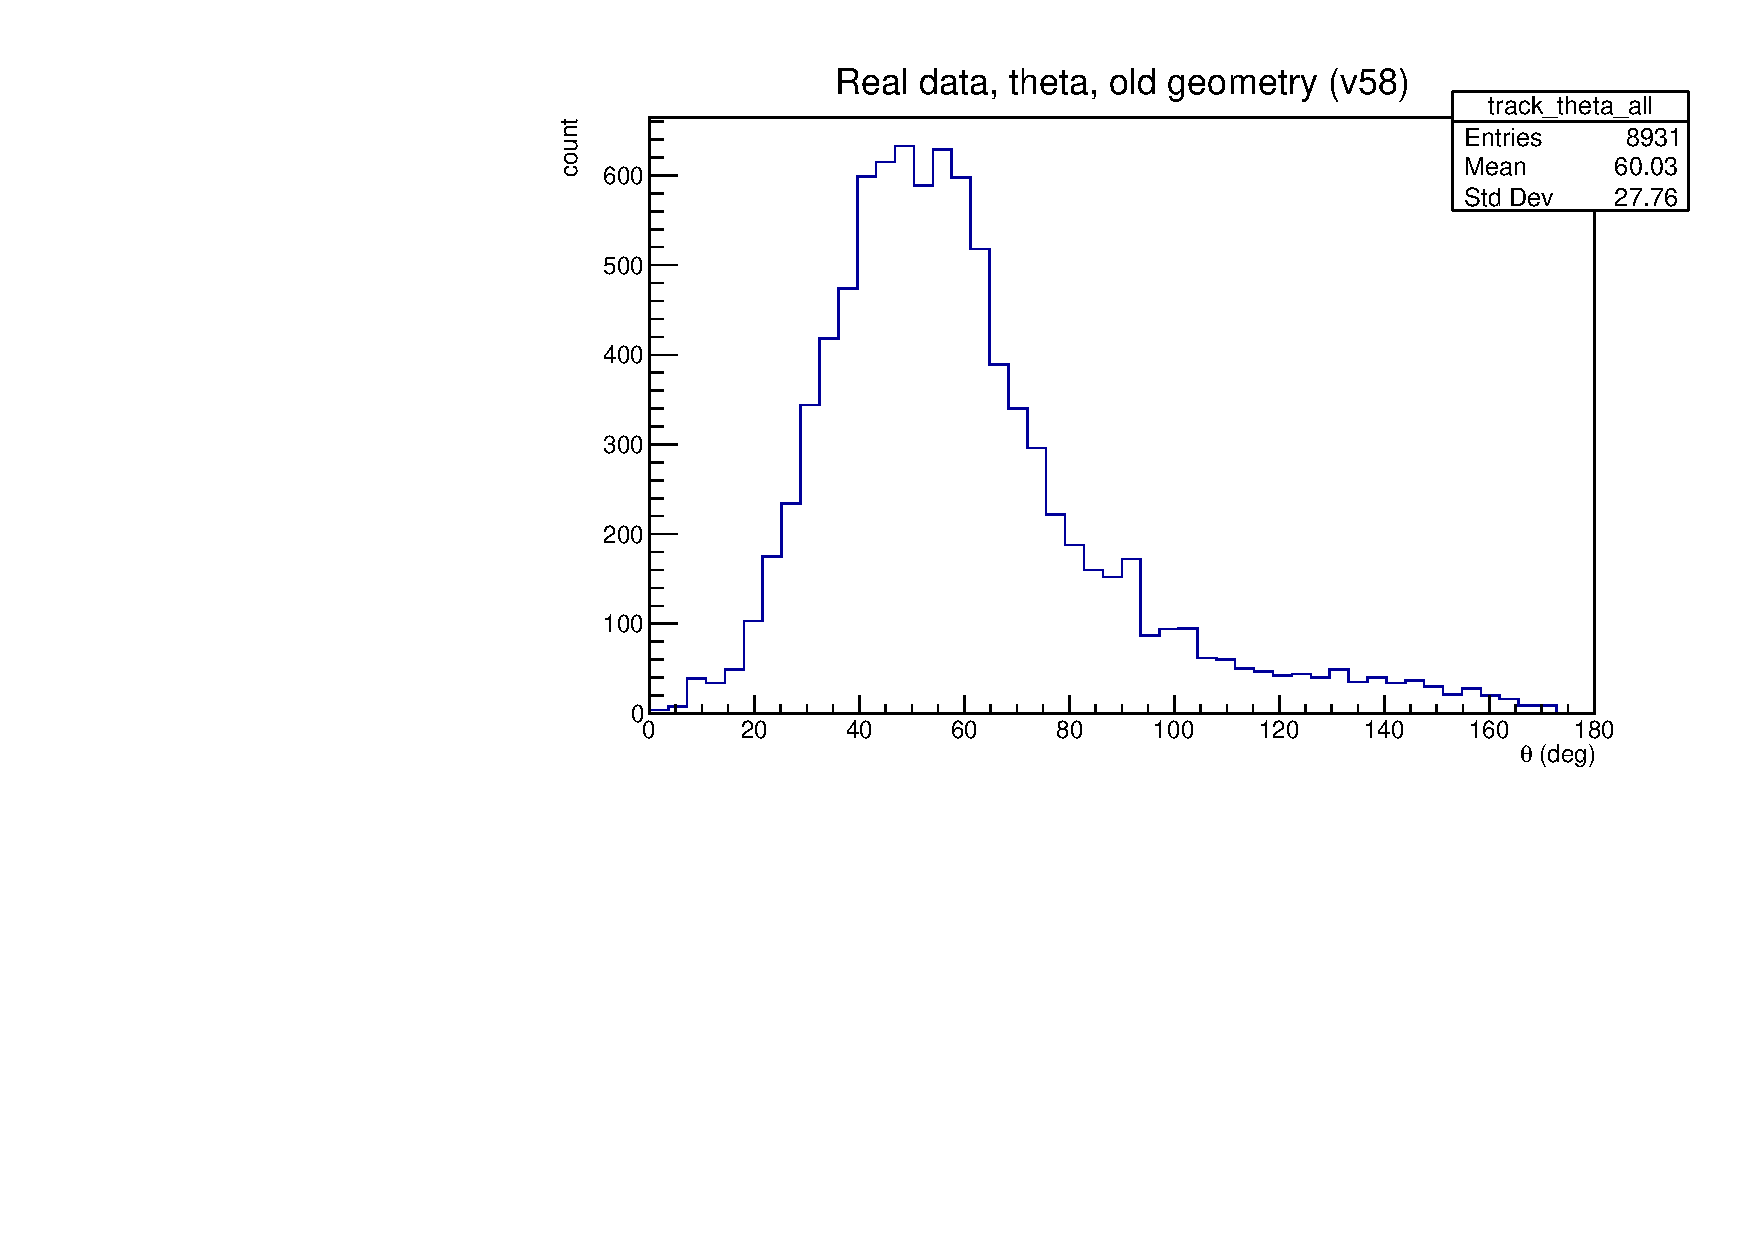
\includegraphics[width=\linewidth]{figures/data_theta_old_geometry.pdf}};
            % Option : système de coordonnées relatif (0 à 1)
            \begin{scope}[x={(image.south east)}, y={(image.north west)}]
                \node [red] at (0.7,0.6) {\tiny before};
            \end{scope}
        \end{tikzpicture}
        \begin{tikzpicture}
            \node[anchor=south west, inner sep=0] (image) at (0,0) {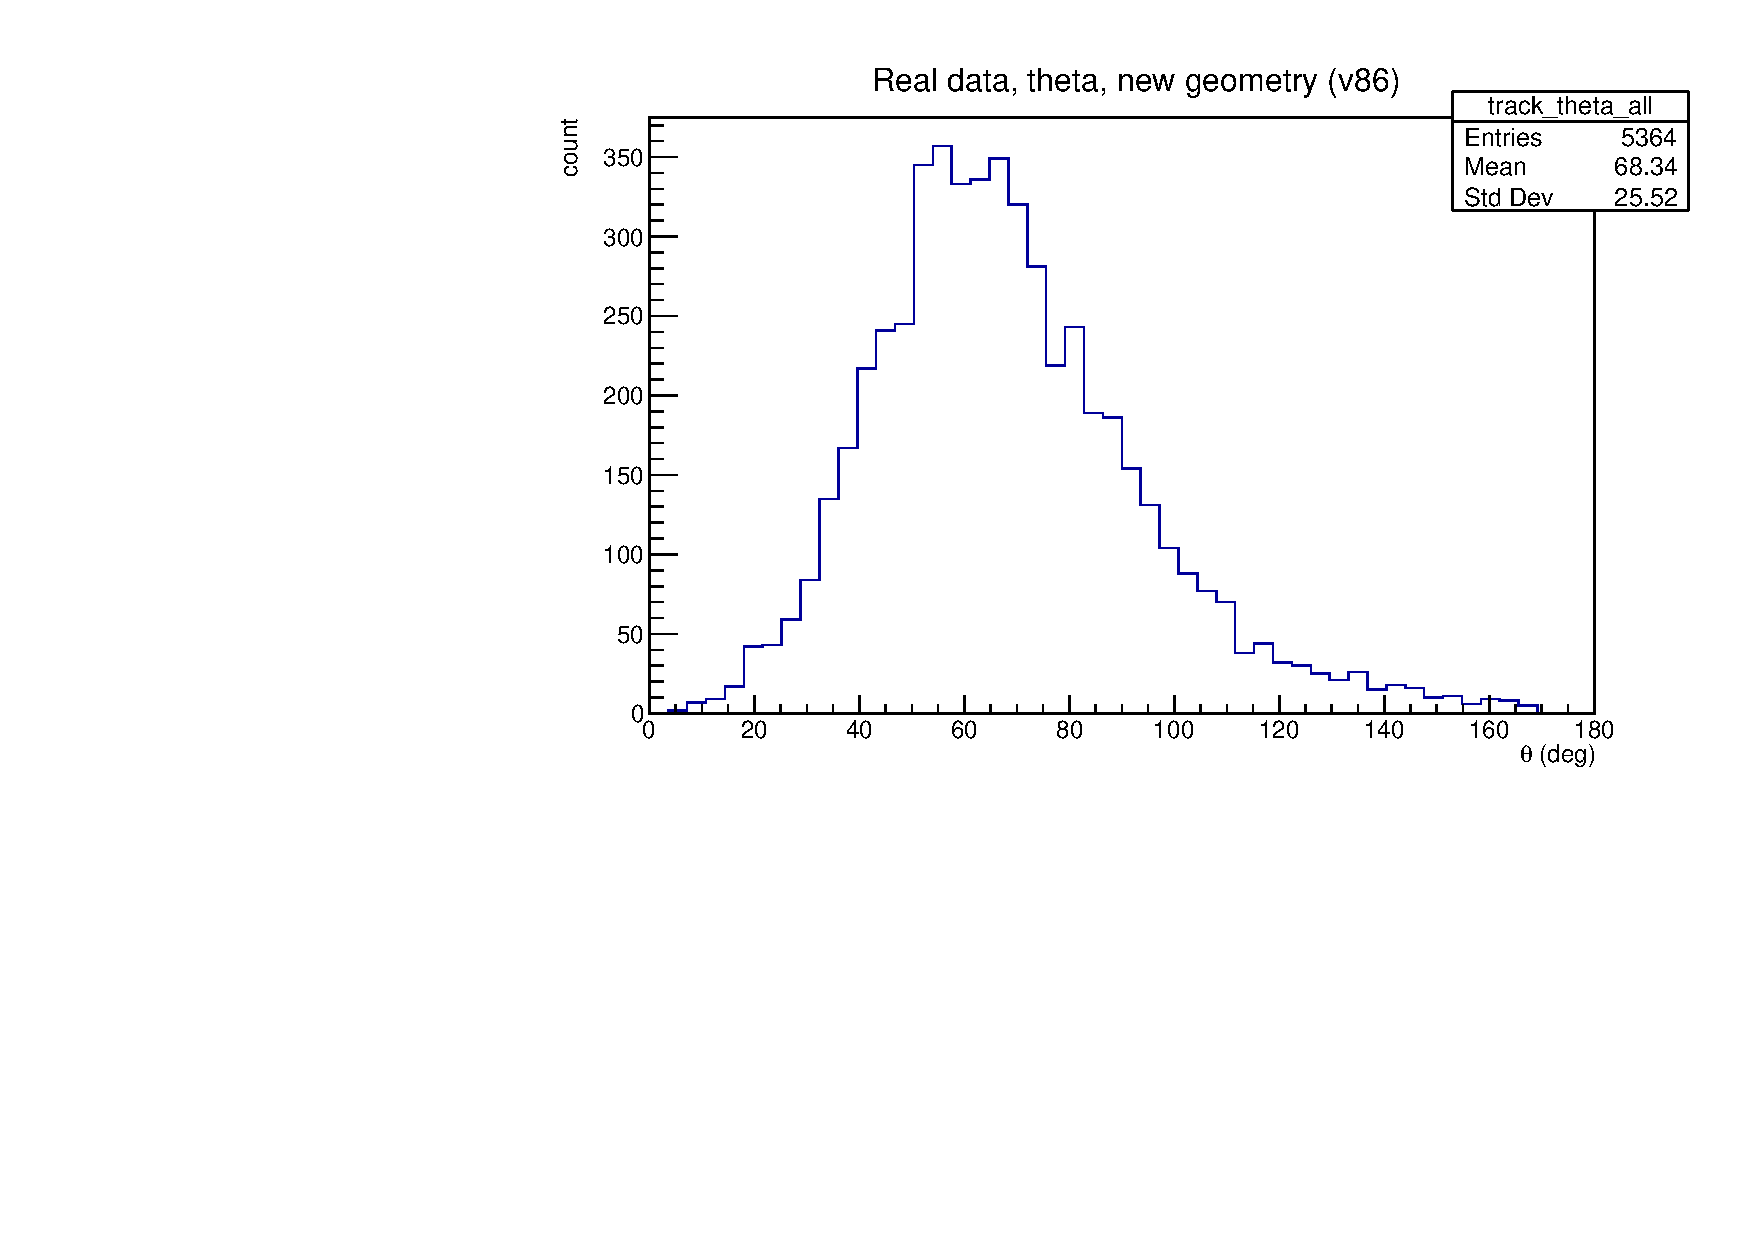
\includegraphics[width=\linewidth]{figures/data_theta_new_geometry.pdf}};
            % Option : système de coordonnées relatif (0 à 1)
            \begin{scope}[x={(image.south east)}, y={(image.north west)}]
                \node [red] at (0.7,0.6) {\tiny after};
            \end{scope}
        \end{tikzpicture}
    \end{minipage}

\end{frame}

\section{Include the ATOF hits in the KF}
\begin{frame}{Include the ATOF hits in the KF 1/3}
    \begin{itemize}
        \item We decided to use the ATOF hits to improve our theta reconstruction
        \item We wanted to use the z position given by the ATOF bars, but their resolutions are not good for the moment. So we used the ATOF wedges instead
        \item The first step was to associate an AHDC track to an ATOF wedge before running the Kalman Filter
    \end{itemize}

    \vspace{0.2cm}

    \centering
    \begin{minipage}{0.75\textwidth}
        \includegraphics[width=\linewidth]{figures/build/atof_hits.pdf}
    \end{minipage}
    

\end{frame}

\begin{frame}{Include the ATOF hits in the KF 2/3}
    \begin{itemize}
        \item We used the work on the ALERT AI track matching presented by Mathieu yesterday \href{https://indico.jlab.org/event/1017/\#72-alert-ai-recon}{(\underline{link} {\scriptsize \faExternalLink*})}.
        %\item However, looking at elastic events, only 30 \% of the tracks found a match in the ATOF.
        \item We also wanted to be able to verify the AI prediction and to find new ATOF wedges based on a track projection
        \item The current strategy is presented in this diagram
        \item The agreement between the AI matching and the projection-based matching is about 70.16 \% (including the $\pm$ 1 indetermination of the wedge)
    \end{itemize}

    \vspace{0.5cm}

    \centering
    \begin{minipage}{0.85\textwidth}
        \includegraphics[width=\linewidth]{figures/build/recon-diagram.pdf}
    \end{minipage}

\end{frame}

\begin{frame}{Include the ATOF hits in the KF 3/3}
    \begin{itemize}
        \item Evolution of the theta reconstruction
        \item We have two peaks in the last version of the theta reconstruction
            \begin{itemize}
                \item The first peak are tracks without ATOF matches
                \item The second peak around 86$^\circ$ are tracks with ATOF matches (45 \%)
            \end{itemize}
        \item The final 45 \% matches (over the nb. tracks) is low; it is essentially due the current misalignment between the AHDC and ATOF
    \end{itemize}

    \vspace{0.5cm}

    \centering
    \begin{minipage}{0.32\textwidth}
        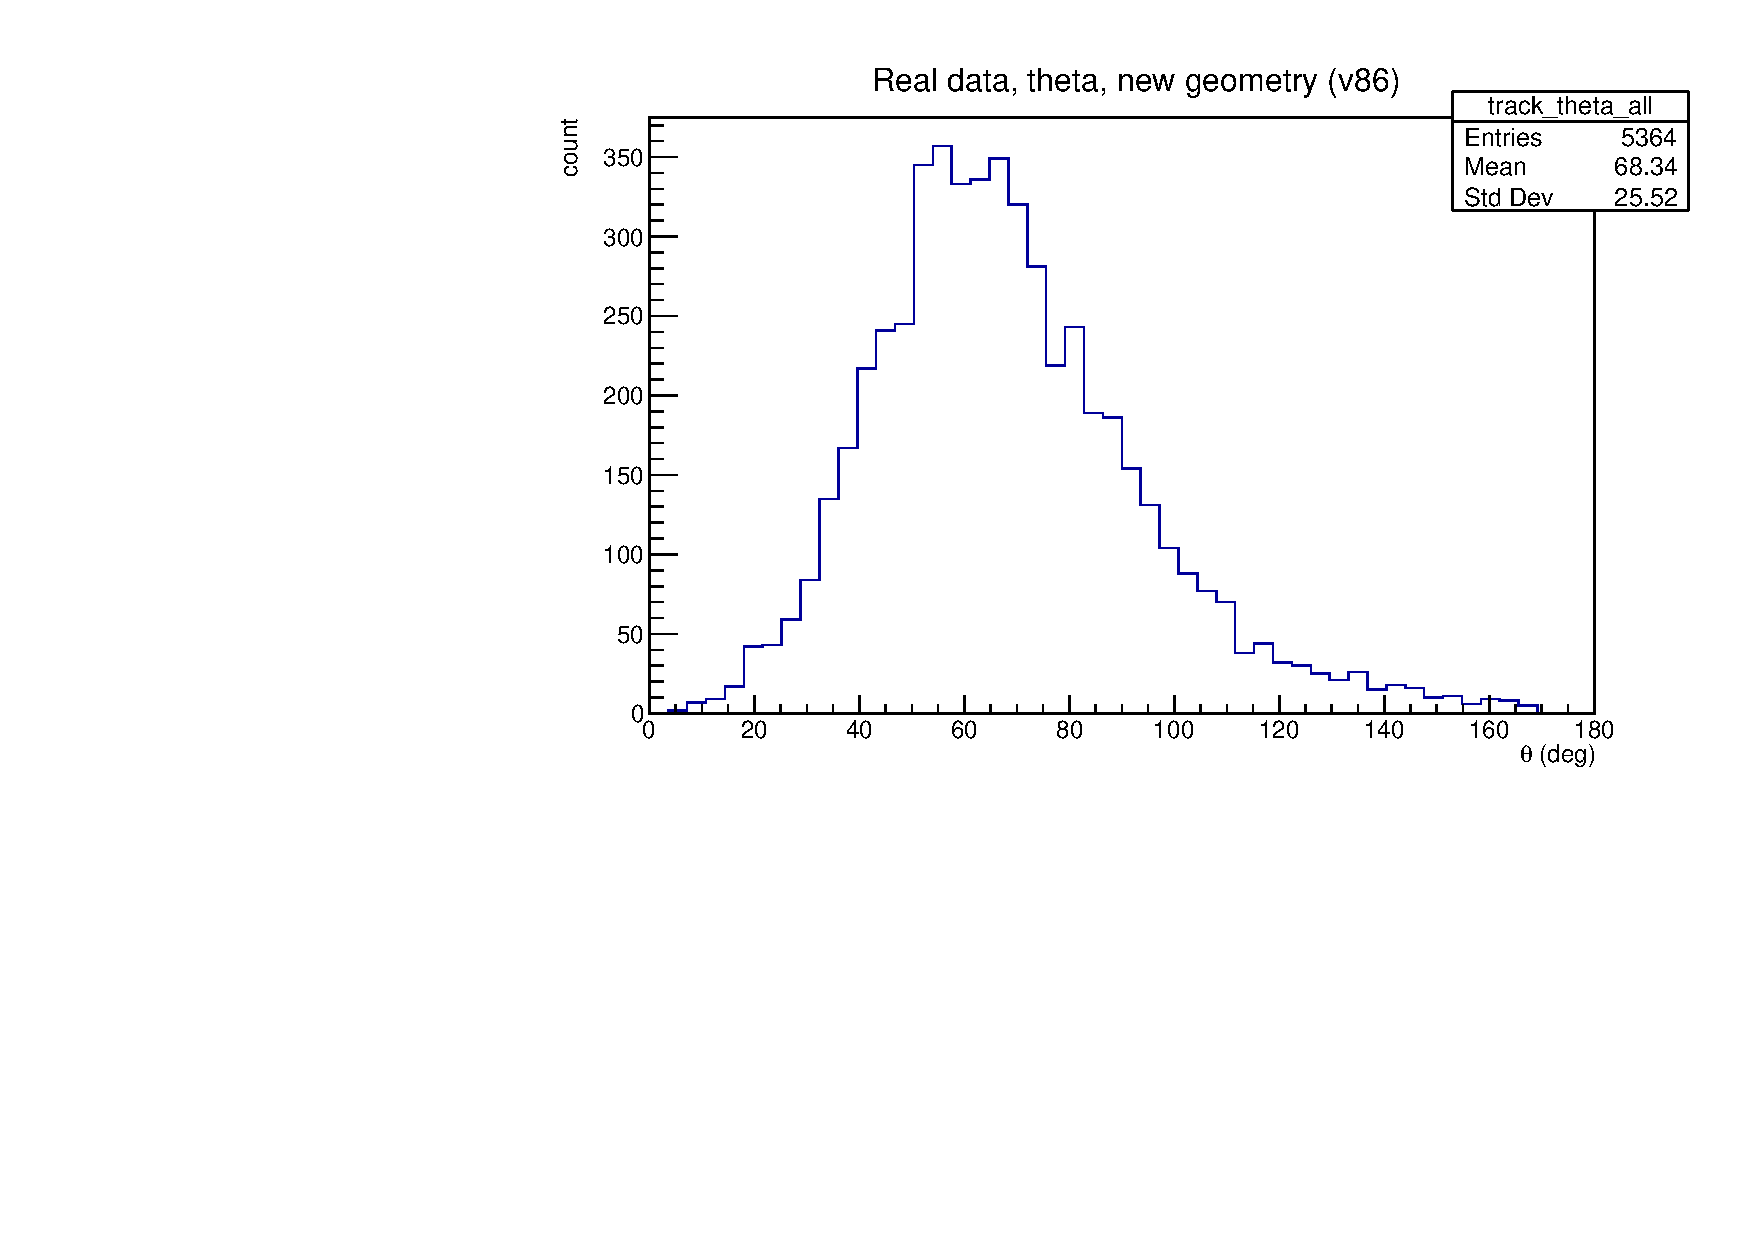
\includegraphics[width=\linewidth]{figures/data_theta_new_geometry.pdf}
    \end{minipage}
    \begin{minipage}{0.32\textwidth}
        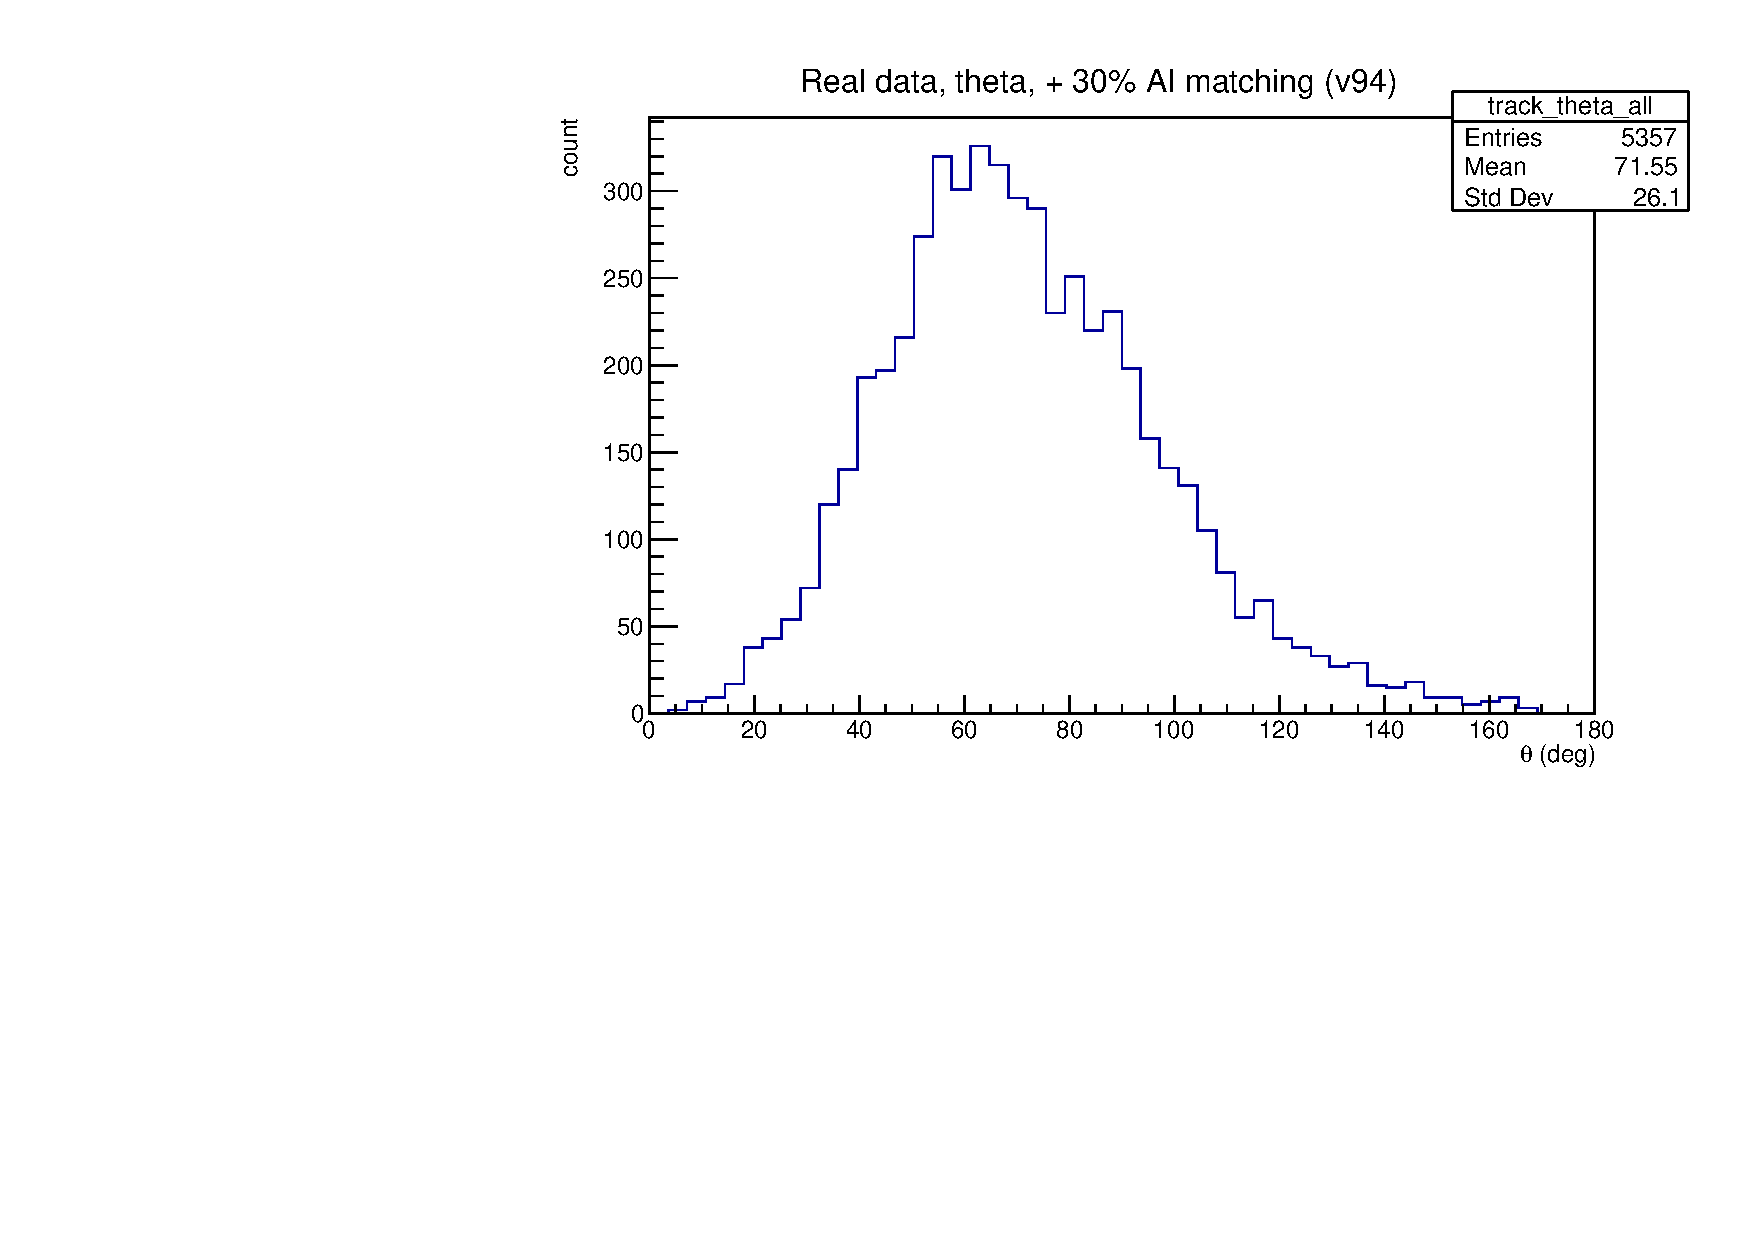
\includegraphics[width=\linewidth]{figures/data_theta_ai_matching.pdf}
    \end{minipage}
    \begin{minipage}{0.32\textwidth}
        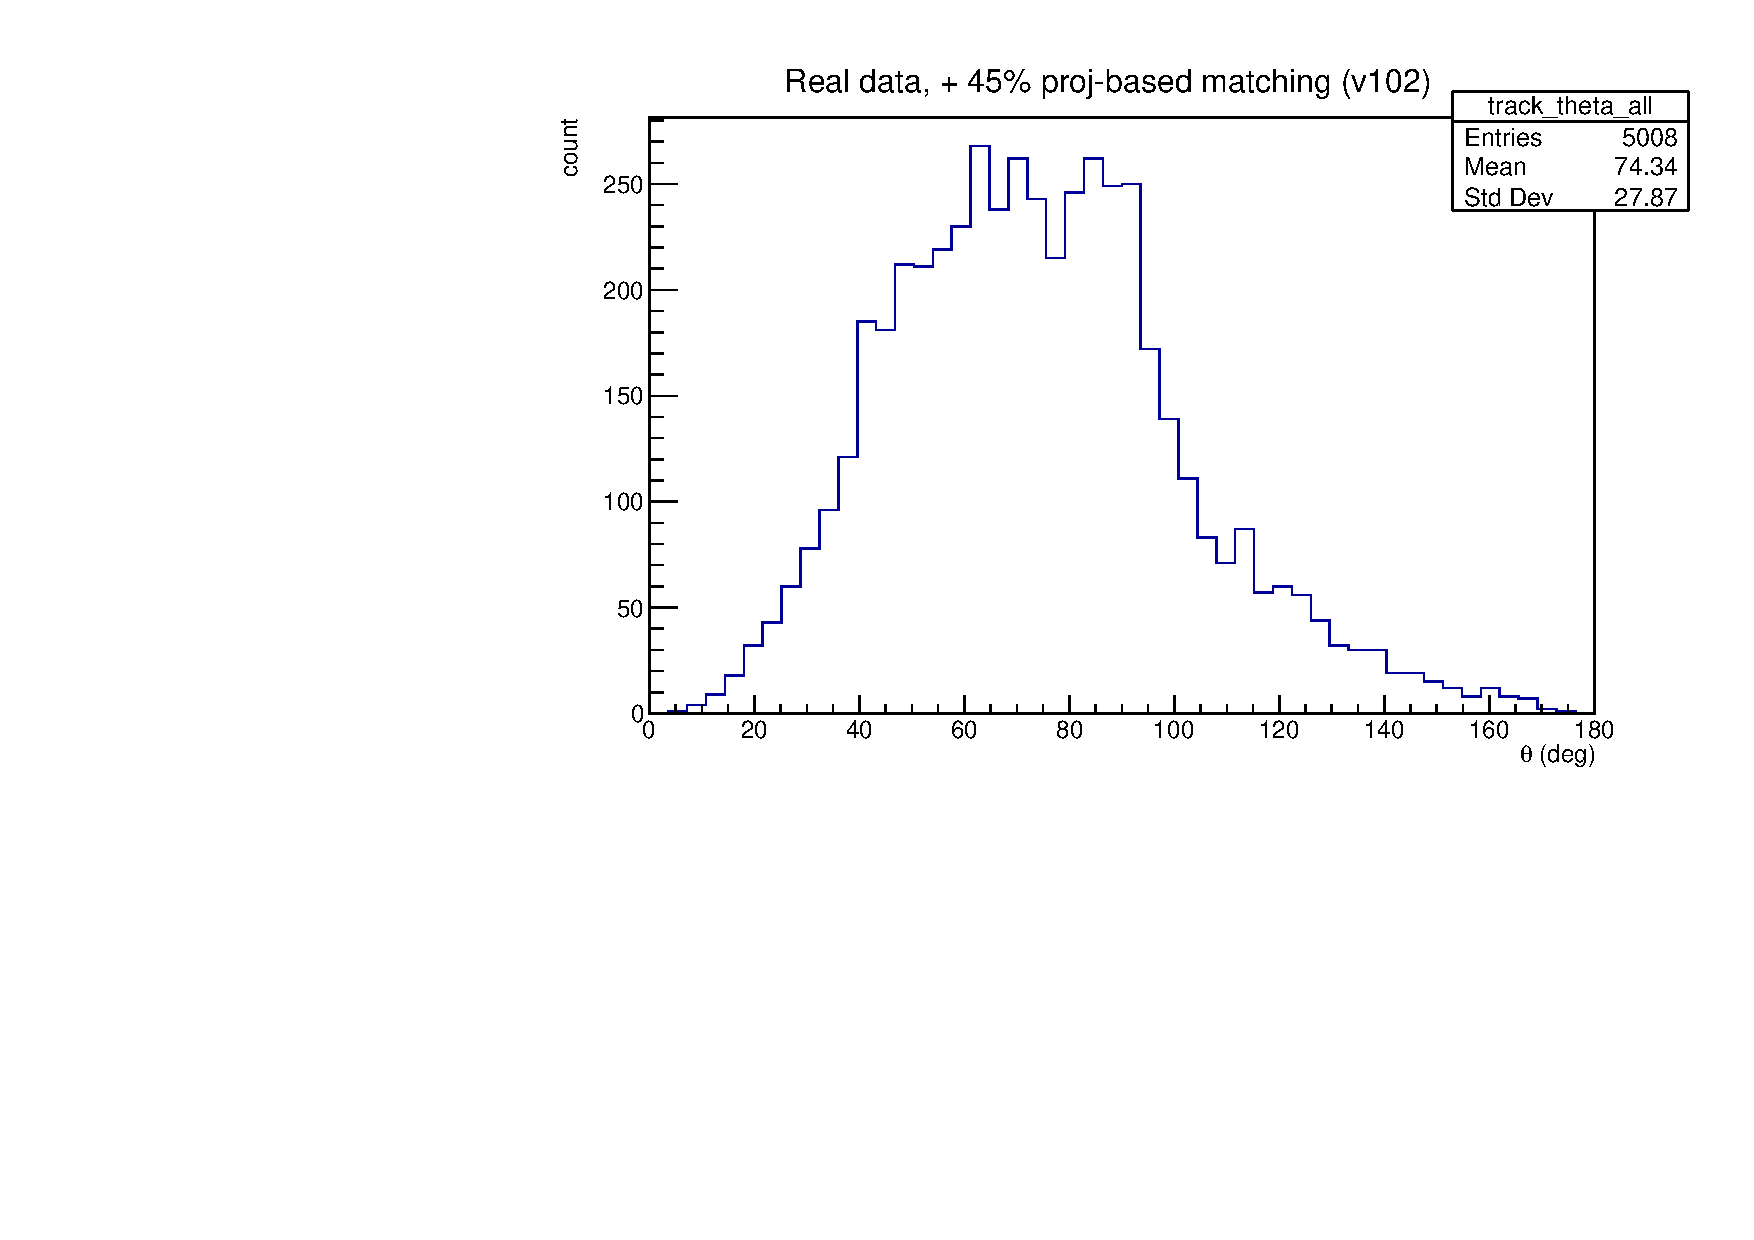
\includegraphics[width=\linewidth]{figures/data_theta_proj_based_matching.pdf}
    \end{minipage}

\end{frame}

\section{Reconstruction status}
\begin{frame}{Reconstruction status}
    \begin{itemize}
        \item dEdx versus p, run 22712 on D2
        \item Elastic cuts: $3.5 \mbox{ GeV}^2 < W^2 < 3.8 \mbox{ GeV}^2$, $|\Delta \phi| < 20^\circ$, $\mbox{nhits} \geq 6$
        \item Hit cleaning included (work on the ATOF hit not included)
    \end{itemize}

    \vspace{0.5cm}

    \centering
    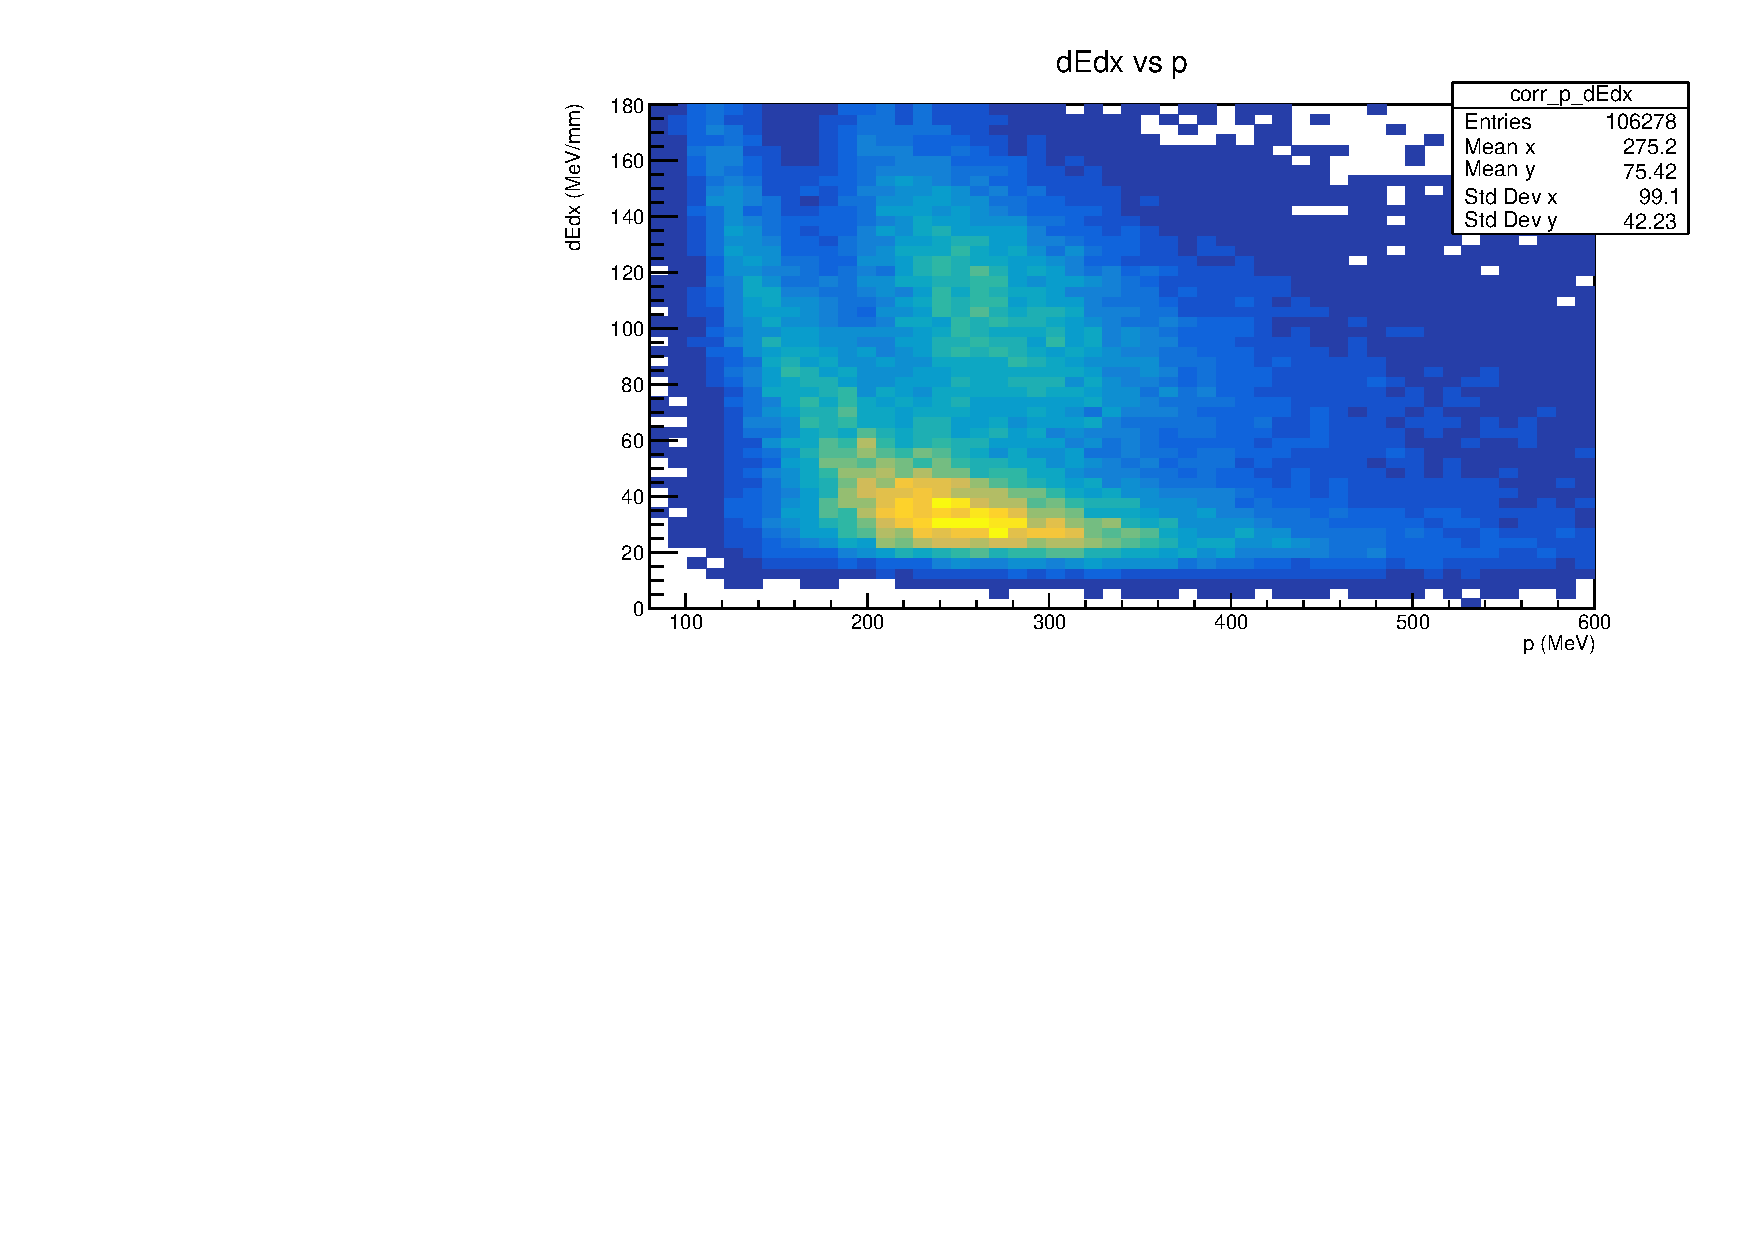
\includegraphics[width=0.8\linewidth]{figures/recon-status-dEdx-versus-momentum.pdf}
\end{frame}

\section{Next steps}
\begin{frame}{Next steps}
    \begin{itemize}
        \item Convenient use of the PID
            \begin{itemize}
                \item For now, the energy loss and the curvature assume the particle to be a proton
                \item We will use the PrePID work of Uditha \href{https://indico.jlab.org/event/1017/\#73-alert-ai-particle-identific}{(\underline{link}) {\scriptsize \faExternalLink*}}
            \end{itemize}
        \item Material verification
            \begin{itemize}
                \item Correct density for the target straw, target gas, ATOF scintillator
                \item Correct use in the Kalman Filter propagator
                \item Vary the density of the AHDC gas with the temperature and the pressure condition over the run period
            \end{itemize}
        \item Fine-tuning
            \begin{itemize}
                \item Electron vertex resolution on $p_e$ and $\theta_e$
                \item Measurement noise of the AHDC hits (ADC and time dependence)
                \item ATOF hits resolution for clusters
                \item Initial error covariance matrix
            \end{itemize}
        \item Work on the AHDC alignment
            \begin{itemize}
                \item With respect to CLAS
                \item With respect to ATOF
            \end{itemize}
    \end{itemize}

    %\vspace{0.5cm}

\end{frame}






\end{document}


